%%%%%%%%%%%%%%%%%%%%%%%%%%%%%%%%%%%%%%
% DOCUMENT CLASS AND GENERAL OPTIONS %
%%%%%%%%%%%%%%%%%%%%%%%%%%%%%%%%%%%%%%
\documentclass[
	parskip, 			   % german paragraph style (no indentation, blank line)
	twoside, 			   % two-sided document
	DIV=14, 			   % narrow margin
	BCOR=15.0mm, 		   % binding correction
	headsepline, 		   % header line
	open=right, 		   % new chapters start on right hand side
	captions=tableheading, % correct distance between table and caption above
	bibliography=totoc,    % references shown in contents
	numbers=noenddot       % remove dots at the the end of chapter numbers
]{scrreprt}

\newcommand{\languages}{english}

\makeatletter
\newcommand\addcase[3]{\expandafter\def\csname\string#1@case@#2\endcsname{#3}}
\newcommand\makeswitch[2][]{%
	\newcommand#2[1]{%
		\ifcsname\string#2@case@##1\endcsname\csname\string#2@case@##1\endcsname\else#1\fi%
	}%
}
\makeatother

\makeswitch[nada]\dothis
\addcase\dothis{english}{\chapter*{Declaration}
\begin{quote}

\vspace*{3cm}

I hereby declare that this thesis is my own work and effort and that it has not been submitted anywhere for any award. Where other sources of information have been used, they have been acknowledged.

\vspace*{2cm}

\begin{flushright}
\underline{\hspace{4cm}}\\
Date\\
\vspace*{1cm}
\underline{\hspace{4cm}}\\
Name
\end{flushright}

\end{quote}

}
\addcase\dothis{ngerman}{\chapter*{Eigenständigkeitserklärung}
\begin{quote}

\vspace*{3cm}

Ich versichere hiermit an Eides statt, dass ich die vorliegende Arbeit selbständig, ohne fremde Hilfe und ohne Benutzung anderer als die angegebenen Hilfsmittel angefertigt habe. Die aus fremden Quellen (einschließlich elektronischer Quellen) direkt oder indirekt übernommenen Gedanken sind ausnahmslos als solche kenntlich gemacht. Die Arbeit ist in gleicher oder ähnlicher Form oder auszugsweise im Rahmen einer anderen Prüfung noch nicht vorgelegt worden.

\vspace*{2cm}

\begin{flushright}
\underline{\hspace{4cm}}\\
Datum\\
\vspace*{1cm}
\underline{\hspace{4cm}}\\
Name
\end{flushright}

\end{quote}

}


%%%%%%%%%%%%%%%%%%%%%%%%%
% PACKAGES AND SETTINGS %
%%%%%%%%%%%%%%%%%%%%%%%%%
\usepackage[utf8]{inputenc} % input umlaut characters directly
\usepackage[T1]{fontenc} % proper output of umlaut characters
\usepackage[ngerman, \languages]{babel} % hyphenation, main language in the end
\usepackage{scrlayer-scrpage} % customise head and foot
\automark[chapter]{chapter} % display chapter name on all pages instead of section name on right hand side
\usepackage{color} % definition of own colors
\definecolor{LTD_grey}{gray}{0.65} % LTD Grau nach dem neuen, druckkostensparenden caltechgray
\addtokomafont{pagehead}{\color{LTD_grey} \sffamily \upshape} % head in grey and sans serif
\addtokomafont{pagenumber}{\color{LTD_grey}} % page number in grey
\addtokomafont{subject}{\normalfont} % Thesis type not bold
\usepackage{graphicx} % scaling of graphics
\usepackage{booktabs} % lines for tabs
\usepackage{amssymb,amsmath} % math symbols
\usepackage{tabularx}
\usepackage{subcaption}
\usepackage{algorithm}
\usepackage{algpseudocode}
\usepackage{hyperref}
\usepackage{minted}
\usepackage{newunicodechar}
\newunicodechar{θ}{$\theta$}
\newunicodechar{α}{$\alpha$}
\newunicodechar{β}{$\beta$}
\newunicodechar{∂}{$\partial$}


%%%%%%%%%%%
% CONTENT %
%%%%%%%%%%%
\begin{document}
\pagenumbering{roman} % roman numbering before main part


%%%%%%%%%%%%%%%%%%%%
% TITLE AND AUTHOR %
%%%%%%%%%%%%%%%%%%%%
\title{On the identification of port-Hamiltonian models via machine-learning} % title
\subject{Master's thesis} % type (Bachelor's thesis / Master's thesis / project thesis)
\author{Jiandong Zhao} % author
 \date{October 2022} % period
 \publishers{supervised by\\[1em]
	Prof. Dr.-Ing. habil. S. Leyendecker\\
	M. Sc. Markus Lohmayer % name of supervisor
	}
\titlehead{
\includegraphics[height=1.45cm]{figures/uni_head_new} \hfill 
\includegraphics[height=1.3cm]{figures/ltd_head}}

% title page
\maketitle


%%%%%%%%%%%%%%%%%%%%%%
% CONTENTS AND LISTS %
%%%%%%%%%%%%%%%%%%%%%%
%% declaration
\dothis{\languages}

% abstract
\chapter*{Abstract}
\begin{quote}

The port-Hamiltonian systems theory provides a port-based modelling approach, with which complex multiphysical systems can be expressed by interconnection of basic components.  The Exergetic Port-Hamiltonian Systems modeling framework combines the classical port-Hamiltonian systems theory with the GENERIC framework, such that exergetic port-Hamiltonian systems are endowed with structural properties, which imply the first and second law of thermodynamics. In the Exergetic Port-Hamiltonian Systems modeling framework, a system consists of subsystems and the environment, where some subsystems may be unknown. In this thesis, we introduce Structured Neural ODEs and use them to construct an IVP. By solving this IVP with numerical method, we obtain the predicted state trajectories. We train neural network models for the subsystems of interest so that these models can be substituted for the subsystems and reused for other systems.

\end{quote}

% contents
\tableofcontents

% figure list
%\listoffigures

% table list
%\listoftables

\cleardoublepage % finish current page with roman numbering


%%%%%%%%%%%%%%%%
% MAIN CONTENT %
%%%%%%%%%%%%%%%%
\pagenumbering{arabic} % arabic numbering for main part


% chapters
\chapter{Introduction}
\label{ch:chapter1}
\section{Motivation}
\section{Main Contributions}
The main contributions of this thesis is two-fold
\section{Outline}
An outline for the following chapters:

\textbf{Chapter} \ref{ch:chapter2} provides a quick overview of ordinary differential equations and initial value problems. It also introduces some numerical methods, in particular a symplectic integrator that will be used in later chapters.

\textbf{Chapter} \ref{ch:chapter3} introduces Hamiltonian systems and port-Hamiltonian systems, since this thesis will focus on modelling physical systems as (port-)Hamiltonian systems.

\textbf{Chapter} \ref{ch:chapter4} gives an introduction to neural networks, which is fundamental for the understanding of later chapters.

\textbf{Chapter} \ref{ch:chapter5} reviews the idea of Neural ODEs. The centre of Neural ODEs is the adjoint method, which is an essential method for data-driven system identification.

\textbf{Chapter} \ref{ch:chapter6} first explores the implementations of priors in the field of physics. Then, it overviews different neural network models for Hamiltonian systems: O-NETs, H-NETs and HNNs. Only O-NET can be used for port-Hamiltonian systems. In addition, structured O-NETs, which are O-NETs endowed with physics priors, are proposed and compared with other neural network models in experiments.

\textbf{Chapter} \ref{ch:chapter7} proposes an approach for modelling (exergetic) port-Hamiltonian systems with structured O-NETs and inplements this approach in experiments.

\textbf{Chapter} \ref{ch:chapter8} draws conclusions and provides an outlook for future work.


\clearpage
\chapter{Differential Equations}
\label{ch:chapter2}

\section{Ordinary Differential Equations}
Consider a real-valued function $x$ with $k$ continuous derivatives: $x \in C^{k}(I)$, where the time interval $ I \subseteq \mathbb{R}, \: k \in \mathbb{N}_{0}, \: x: \mathbb{R} \rightarrow \mathbb{R}$. An implicit ordinary differential equation (ODE) is a functional relation of the form:

\begin{equation}
    \label{eq:implicit_ODE}
    F\left(t, x, x^{(1)}, \ldots, x^{(k)}\right)=0.
\end{equation}

We assume that the highest order derivative $x^{(k)}$ is solvable, and placing it on the left hand side alone, it becomes the explicit ordinary differential equation of the form:

\begin{equation}
    \label{eq:explicit_ODE}
    x^{(k)} = F\left(t, x, x^{(1)}, \ldots, x^{(k-1)}\right).
\end{equation}

More general, consider the case $x: I \rightarrow \mathbb{R}^{n}$. Equation \ref{eq:explicit_ODE} can be extended to a system of ordinary differential equations:

\begin{equation}
    \label{eq:ODE_system}
    \begin{aligned}
    x_{1}^{(k)} &=F_{1}\left(t, x, x^{(1)}, \ldots, x^{(k-1)}\right) \\
    x_{2}^{(k)} &=F_{2}\left(t, x, x^{(1)}, \ldots, x^{(k-1)}\right) \\
    & \vdots \\
    x_{n}^{(k)} &=F_{n}\left(t, x, x^{(1)}, \ldots, x^{(k-1)}\right).
\end{aligned}
\end{equation}

The above form is a N-dimensional system, which has $N$ ordinary differential equations. Commonly, $t$ is called the independent variable and $x$ is called the dependent variable.

\section{Initial Value Problems}
An initial value problem (IVP) consists of an explicit ODE (or a system of ODEs) and an initial state:

\begin{equation}
    \label{eq:IVP}
    \dot{x} = f(t, x), \quad x(t_{0})=x_{0}.
\end{equation}

By integrating both sides of the explicit ODE, we obtain an integral equation of the form:

\begin{equation}
    \label{eq:solution_IVP}
    x(t) = x_{0} + \int_{t_{0}}^{t} f(s, x(s))\:ds.
\end{equation}

Take a small step from $t_{0}$ to $t_{0}+\Delta t$, then $x_{1}$ can be computed by:

\begin{equation}
    \label{eq:solution_IVP_first_step}
    x_{1} = x_{0} + \int_{t_{0}}^{t_{0}+\Delta t} f(s, x(s))\:ds.
\end{equation}

In the same way, $x_{2}$ can be computed by:

\begin{equation}
    \label{eq:solution_IVP_second_step}
    x_{2} = x_{1} + \int_{t_{1}}^{t_{1}+\Delta t} f(s, x(s))\:ds.
\end{equation}

Suppose that the time evolution ends with $T$, by repeating the above procedure, we obtain a sequence of approximating solutions $ \{ x_t \}_{0}^{T}$. In dynamical systems, $\{ x_t \}_{0}^{T}$ is a  set of points in state space, which is also known as state trajectory.


\clearpage
\section{Numerical Methods}
In this section, we discuss some numerical methods for solving IVPs. We refer to the solutions provided by numerical methods as numerical solutions. Although numerical methods provide approximations rather than exact solutions, they are widely implemented because they can be used in computer programs. In addition, the algorithmic descriptions regarding numerical methods are known as numerical schemes.

\subsection{Explicit Euler Method}
The Euler method is the simplest and probably the first numerical method formulated by Leonhard Euler in 1768. Consider an IVP problem such as \ref{eq:IVP}. The explicit Euler method is of the form

\begin{equation}
    \label{eq:Eulers_method_explicit}
    y_{n+1} = y_{n} + h \cdot f_{n},
\end{equation}

where h is the step step $h = t_{n+1} - t_{n}$ and $f_{n}$ is the time derivative of $y$ at time $t_{n}$, i.e. $f_{n} = f(y_n, t_n) = \left. \frac{dy}{dt} \right|_{t=t_n}$.

\subsection{Implicit Euler Method}
The implicit Euler method is of the form

\begin{equation}
    \label{eq:Eulers_method_implicit}
    y_{n+1} = y_{n} + h \cdot f_{n+1},
\end{equation}

where $f_{n+1} = f(y_{n+1}, t_{n+1}) = \left. \frac{dy}{dt} \right|_{t=t_{n+1}}$. Comparing to the explicit form \ref{eq:Eulers_method_explicit}, the solution $y_{n+1}$ is defined implicitly. Hence, to obtain the solution of an IVP by using such an implicit method, we need to solve a system of nonlinear equations.

\subsection{Implicit Midpoint Rule}
The implicit midpoint is of the form

\begin{equation}
    \label{eq:Midpoint_rule_implicit}
    y_{n+1} = y_{n} + h \cdot f(t_{n}+\frac{h}{2} ,\frac{y_{n} + y_{n+1}}{2}),
\end{equation}

where $f$ evaluates the slope of the solution at time $t_{n}+\frac{h}{2}$.

The implicit midpoint rule is a symplectic integrator. In contrast to \ref{eq:Eulers_method_explicit} and \ref{eq:Eulers_method_implicit}, this symplectic integrator allows the solution trajectory to remain unchanged after inverting the direction. In more detail, after exchanging $y_{n+1}$ and $y_{n}$, the form \ref{eq:Midpoint_rule_implicit} can be rewritten as

\begin{equation}
    \label{eq:Midpoint_rule_implicit_inverted}
    y_{n} = y_{n+1} + h \cdot f(t_{n}+\frac{h}{2} ,\frac{y_{n} + y_{n+1}}{2}).
\end{equation}

Such an inversion only changes the direction of the solution trajectory but does not affect the solution trajectory itself. This property of the symplectic integrator makes it useful for some reversible systems, such as Hamiltonian systems.

\clearpage
\chapter{Port-Hamiltonian Systems}
\label{ch:chapter3}

\section{Hamiltonian Systems}

\subsection{Formulation}
In general, a Hamiltonian system is a triple $(\mathcal{X},\omega,H)$, where $(\mathcal{X},\omega)$ is a symplectic manifold which consists of a manifold $\mathcal{X}$ and a symplectic structure or a symplectic form $\omega$. The Hamiltonian or Hamiltonian function $H: \mathcal{X} \mapsto \mathbb{R} $ is a smooth function on the manifold $\mathcal{X}$, i.e., $H \in C^{\infty}(\mathcal{X})$ \cite{rudolph2017differential}. And the unique Hamiltonian vector field corresponding to the Hamiltonian function $H$ is denoted by $X_H = \{H, \cdot \}$, where $\{\cdot, \cdot\}$ is a possion bracket. Suppose that the possion bracket is on the symplectic manifold $(\mathcal{X},\omega)$ and a smooth function is on the manifold $\mathcal{X}$, i.e., $f \in C^{\infty}(\mathcal{X}) $. Thus, the evolution of $f$ can be given by $\dot{f} = \{H, f\} = X_H(f)$. For more details, we refer to \cite{rudolph2012differential}.

In this thesis, we restrict our study to autonomous systems. In mechanical systems, the Hamiltonian can be formulated by $H(\mathbf{q},\mathbf{p})=T(\mathbf{q},\mathbf{p})+V(\mathbf{q})$, where $T(\mathbf{q},\mathbf{p})$ is the kinetic energy and $V(\mathbf{q})$ is the potential energy of the system. With the generalized coordinate $\mathbf{q} = (q^1, q^2, ..., q^n)$ and generalized momentum $\mathbf{p} = (p_1, p_2, ..., p_n)$, the Hamiltonian is of the form

\begin{equation}
    \label{eq:Hamiltonian}
    H(\mathbf{q},\mathbf{p})=\frac{1}{2}\mathbf{p}^T\mathbf{M}^{-1}(\mathbf{q})\mathbf{p} + \mathbf{V}(\mathbf{q}),
\end{equation}

where $\mathbf{M}^{-1}(\mathbf{q})$ is the mass matrix, which expresses the inertia of the system.

\subsection{Dynamics}
We use canonical coordinates $q^i$ and $p_i$, which are sets of coordinates in phase space, to describe the Hamiltonian systems. Consider $q^i$ and $p_i$ are smooth functions on the manifold $\mathcal{X}$, i.e., $q^i \in C^{\infty}(\mathcal{X})$ and $p_i \in C^{\infty}(\mathcal{X})$. Recall that the possion bracket $\{H, f\}$ is on the symplectic manifold $(\mathcal{X},\omega)$. Hence, the Hamiltonian vector field can be written as 

\begin{equation}
    \label{eq:Hamiltonian_vector_field}
    X_H = \sum\nolimits_{i=1}^n \frac{\partial H}{\partial p_i} \frac{\partial}{\partial q^i} - \frac{\partial H}{\partial q^i} \frac{\partial}{\partial p_i}.
\end{equation}

We also refer to the Hamiltonian vector field $X_H$ as the symplectic gradient of $H$.

Then, the dynamcis of the Hamiltonian systems is given by 

\begin{equation}
    \label{eq:Hamiltonian_dynamcis}
    \begin{aligned}
    \dot{q}^i &= \{H, q^i\} = X_H(q^i)=\frac{\partial H}{\partial p_i},\\
    \dot{p}_i &= \{H, p_i\}= X_H(p_i)=-\frac{\partial H}{\partial q^i}.
    \end{aligned}
\end{equation}


\subsection{Conservation of Energy}
Let the state variables $\mathbf{x}=(\mathbf{q},\mathbf{p}) \in \mathcal{X}$. If a Hamiltonian is time-independent, it holds

\begin{equation}
    \label{eq:Hamiltonian_invariant}
    \frac{dH}{dt} = (\frac{\partial H}{\partial \mathbf{x}})^T \frac{d\mathbf{x}}{dt} = 0,
\end{equation}

where the time derivatives of the state variables can be written in the form:

\begin{equation}
    \label{eq:Hamiltonian_symplectic}
    \begin{aligned}
        \frac{d\mathbf{x}}{dt} &= J \frac{\partial H}{\partial \mathbf{x}},\\\\
        \text{where}\\
        J &= \left[ \begin{array}{cc}
            0 & -I \\
            I & 0
        \end{array} \right]
    \end{aligned}.
\end{equation}

A matrix $J$ that holds $-J = J^T$ is called skew-symmetric matrix.

Plugging \ref{eq:Hamiltonian_symplectic} into \ref{eq:Hamiltonian_invariant}, we can prove that the Hamiltonian is conserved:

\begin{equation}
    \label{eq:Hamiltonian_symplectic_conclusion}
    \begin{aligned}
        \frac{dH}{dt} &= (\frac{\partial H}{\partial \mathbf{x}})^T \frac{d\mathbf{x}}{dt}\\
         &= (\frac{\partial H}{\partial \mathbf{x}})^T J \frac{\partial H}{\partial \mathbf{x}} \\
         &= 0.
    \end{aligned}
\end{equation}


In addition to using skew-symmetric matrix in general systems, in a mechanical system such as \ref{eq:Hamiltonian}, the conservation law is of the form:

\begin{equation}
    \label{eq:Hamiltonian_invariant_in_mechaniacal_system}
    \frac{dH}{dt} = \frac{\partial H}{\partial \mathbf{q}} \frac{d \mathbf{q}}{dt} + \frac{\partial H}{\partial \mathbf{p}} \frac{d \mathbf{p}}{dt} = 0.
\end{equation}

\subsection{Symplectic Integration of Hamiltonian Systems}
Plugging \ref{eq:Hamiltonian_symplectic} into the symplectic integrator \ref{eq:Midpoint_rule_implicit}, we obtain:

\begin{equation}
    \label{eq:Midpoint_rule_implicit_Hamiltonian}
    y_{n+1} = y_{n} + h \cdot J \nabla H (t_{n}+\frac{h}{2} ,\frac{y_{n} + y_{n+1}}{2}).
\end{equation}

The differentiation of $y_{n+1}$ with respect to $y_{n}$ yields

\begin{equation}
    \label{eq:Midpoint_rule_implicit_Hamiltonian_differentiation}
    (I - \frac{1}{2} h \cdot J \nabla^2 H) \frac{y_{n+1}}{y_{n}} = (I + \frac{1}{2} h \cdot J \nabla^2 H).
\end{equation}

We can prove that

\begin{equation}
    \label{eq:Midpoint_rule_implicit_symplecticity}
    (\frac{y_{n+1}}{y_{n}})^T J (\frac{y_{n+1}}{y_{n}}) = J.
\end{equation}

The relation \ref{eq:Midpoint_rule_implicit_symplecticity} satisfy for all $t$. A linear mapping $A: \mathbb{R}^2n \mapsto \mathbb{R}^2n$ is called symplectic if $A^T J A = J$. Hence, we say $y_{n+1}$ is a symplectic transformation and \ref{eq:Midpoint_rule_implicit_Hamiltonian} is a symplectic integrator.


\subsection{Example: Undamped Harmonic Oscillator}
An undamped harmonic oscillator is a classical Hamiltonian system. A mass $m$ is connected to one end of a spring with compliance $c$ and the other end of the spring is fixed. The direction of the displacement $q$ is positive in the direction of being stretched by the mass.

\clearpage
\begin{figure}[h!]
    \centering
    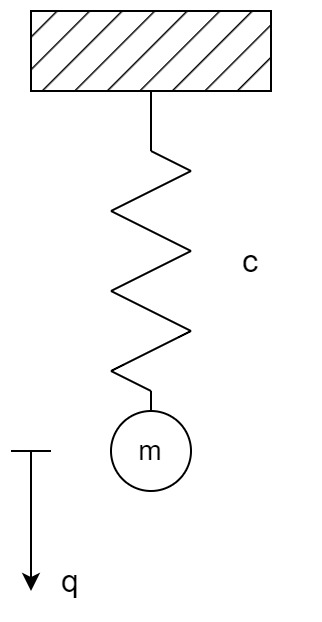
\includegraphics[scale=0.3]{figures/undamped harmonic oscillator.jpg}
    \caption{Undamped harmonic oscillator.}
    \label{fig:physical_model_undamped_harmonic_oscillator}
\end{figure}

In Newtonian mechanics, according to Newton's second law $F=ma=m\ddot{x}$ and Hooke's law $F_s=kx$ ($F_s$ is the restoring force of a spring, which is always in the opposite direction to the displacement), it holds $m\ddot{x}+kx=0$, which is an implicit ODE in the form of equation \ref{eq:implicit_ODE}. As the highest order in the ODE is second order, it is called second order differential equation.

In Hamiltonian mechanics, referring to equation \ref{eq:Hamiltonian}, the Hamiltonian is the sum of the kinetic energy $\frac{1}{2}\mathbf{p}^T\mathbf{M}^{-1}(\mathbf{q})\mathbf{p}$ and the potential energy $\mathbf{V}(\mathbf{q})$. In the case of undamped harmonic oscillator, this can be rewritten as

\begin{equation}
    \label{eq:Hamiltonian_udho}
    H(q,p)=\frac{1}{2c}q^2+\frac{1}{2m}p^2,
\end{equation}

where p is the momentum of the mass. The state of the system (in canonical coordinates) $x=(q,p)$ moves along the Hamiltonian vector field $X_{H}=\{H, \cdot\}$, where the possion bracket is on the symplectic manifold $(\mathcal{X},\omega)$. According to \ref{eq:Hamiltonian_vector_field}, the evolution of $q$ and $p$ can be given by

\begin{equation}
    \label{eq:ODE_undamped_harmonic_oscillator}
    \begin{aligned}
        \dot{q}&=X_{H}(q)=\frac{\partial H}{\partial p}=\frac{p}{m},\\
        \dot{p}&=X_{H}(p)=-\frac{\partial H}{\partial q}=-\frac{q}{c}.
    \end{aligned}
\end{equation}

Moving along the Hamiltonian vector field keeps the total energy of a Hamiltonian system constant. In this way, the time derivative of Hamiltonian stays at zero:

\begin{equation}
    \label{eq:derivative_Hamiltonian}
    \dot{H}=\frac{\partial H}{\partial q}\dot{q}+\frac{\partial H}{\partial p}\dot{p}=0.
\end{equation}


\section{Port-Hamiltonian Systems}
The port-Hamiltonian systems formulation provides a port-based modelling approach, where a complex system can be expressed by an interconnection of several components. In this thesis, we use a bond-graph expression, which is based on the bond-graph theory \cite{paynter1961analysis}, to provide graphical representation of port-Hamiltonian systems.

\subsection{Dirac Structure}
The centre of port-Hamiltonian systems is a Dirac structure defined by

\begin{equation}
    \label{eq:Dirac_structure}
    \mathcal{D}_x \subset T_{x}\mathcal{X} \times T_{x}^{*}\mathcal{X} \times \mathcal{F}_R \times \mathcal{E}_R \times \mathcal{F}_P \times \mathcal{E}_P,
\end{equation}

where the pair $(f_S, e_S) \in T_{x}\mathcal{X} \times T_{x}^{*}\mathcal{X}$ is the energy-storing port, the pair $(f_R, e_R) \in \mathcal{F}_R \times \mathcal{E}_R$ is the energy-dissipating port and the pair $(f_P, e_P) \in \mathcal{F}_P \times \mathcal{E}_P$ is the external port.

As can be seen in \ref{eq:Dirac_structure}, a Dirac structure is a subspace $\mathcal{D} \subset \mathcal{F} \times \mathcal{E}$, where $\mathcal{F}$ and $\mathcal{E}$ are the spaces of the port variables (i.e. flows $f$ and efforts $e$). We refer to a pair $(f,e)$ of vectors of flow and effort variables as a port. In port-Hamiltonian systems, the subsystems interact with each other via ports. Such interactions are assumed to be the exchanges of energy.

\subsection{Example: Isothermal Damped Harmonic Oscillator}
Unlike the previous example, the mechanical energy of an isothermal damped harmonic oscillator dissipates with the vibration.

\clearpage
\begin{figure}[h!]
    \centering
    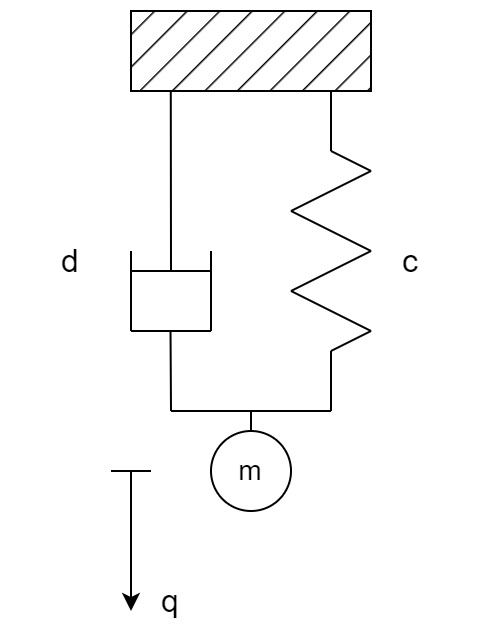
\includegraphics[scale=0.3]{figures/isothermal damped harmonic oscillator.jpg}
    \caption{Isothermal damped harmonic oscillator.}
    \label{fig:idho}
\end{figure}

Figure \ref{fig:idho} illustrates an isothermal damped harmonic oscillator, where $d$ is the damping coefficient.

This system can also be depicted by a bond-graph expression. To distinguish different types of subsystems more visually, storage components are shown in blue, Dirac structures in green and resistive structures in red:

\begin{figure}[h!]
    \centering
    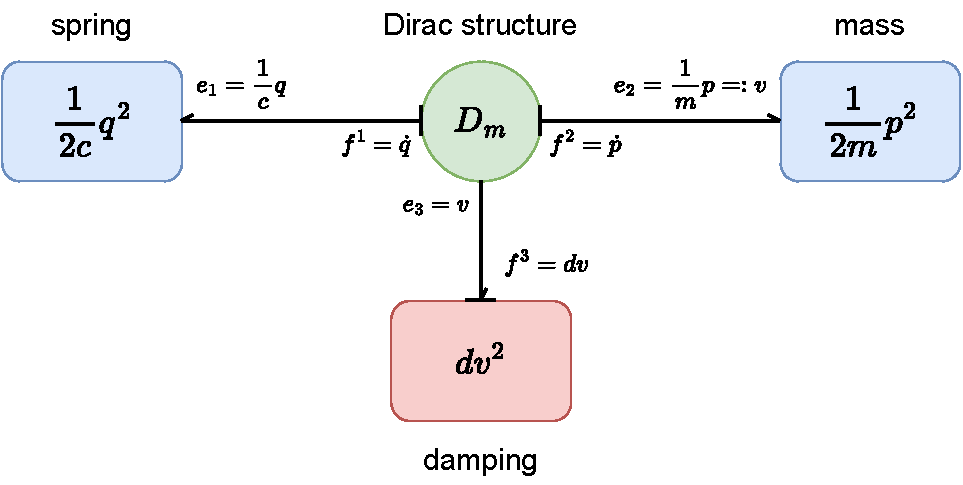
\includegraphics[scale=0.8]{figures/bondgraph_idho.pdf}
    \caption{Bond-graph expression for isothermal damped harmonic oscillator. The strokes perpendicular to the bond and adjacent to the subsystems are called causal strokes, which mark the causality between the subsystems and the flow variables. For instance, we say that $D_m$ causes $f^1$.}
    \label{fig:bondgraph_idho}
\end{figure}



\textbf{The storage components} spring and mass are connected to the Dirac structure $D_m$ via ports 
$(f^1, e_1) = (\dot{q}, \partial_q H)$ and $(f^2, e_2) = (\dot{p}, \partial_p H)$.

\textbf{The resistive structure} damping is connected to the Dirac structure $D_m$ via port $(f^3, e_3) = (dv, v)$. Note that the velocity $v$ is $p/m$. According to the prerequisite "isothermal", the damping will not exchange energy with the environment. Hence, the net power at the damping $e_3 f^3 = dv^2$ represents the dissipated energy of the system.

\textbf{The Dirac structure $D_m$} can be defined by:

\begin{equation}
    \label{eq:Dirac_structure_idho}
    \mathcal{D}_m=\left\{ \left( \left[\begin{array}{l}f^1 \\ f^2 \\ \hline f^3 \end{array} \right], \left[\begin{array}{l} e_1 \\ e_2 \\ \hline e_3 \end{array}\right] \right) \in \mathcal{F} \times \mathcal{E}    \,\middle\vert\,    \left[\begin{array}{l}f^1 \\ f^2 \\ \hline e_3\end{array}\right]=J\left[\begin{array}{l}e_1 \\ e_2 \\ \hline f^3 \end{array}\right]\right\},
\end{equation}

where $J$ is a skew-symmetric matrix

\begin{equation}
    \label{eq:skew-symmetric_matrix_idho}
    \left[\begin{array}{rr|r}
    0 & 1 & 0 \\
    -1 & 0 & -1 \\
    \hline 0 & 1 & 0
    \end{array}\right].
\end{equation}

We can also reformulate the interconnection from \ref{eq:Dirac_structure_idho} and obtain the dynamics by canonical coordinates:

\begin{equation}
    \label{eq:ODE_isothermal_damped_harmonic_oscillator}
    \begin{bmatrix}
    \dot{q}\\
    \dot{p}\\
    \end{bmatrix}
    =
    \begin{bmatrix}
    \frac{p}{m}\\
    -\frac{q}{c}-d\frac{p}{m}\\
    \end{bmatrix}.
\end{equation}


\clearpage
\chapter{Neural Networks}
\label{ch:chapter4}
Artificial neural networks (ANNs), also referred to simply as neural networks (NNs), are algorithmic models that mimic the behavioral characteristics of animal neural networks for distributed parallel information processing, even though this mimicry is superficial \cite{russell2010artificial}. Such networks rely on the complexity of the system to process information by adjusting the relationship between a large number of internal nodes connected to each other.

\section{Perceptron}
Neural network technology originated in the 1950s as perceptron by McCulloch and Pitts \cite{mcculloch1943logical}. The characteristics of perceptrons are strongly contemporary: their inputs and outputs are in binary form. Each of these perceptrons is characterized as either "on" or "off", with an "on" response occurring when stimulated by a sufficient number of neighboring perceptrons.

\begin{figure}[h!]
    \centering
    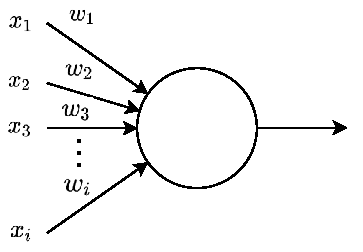
\includegraphics[scale=1]{figures/perceptron.pdf}
    \caption{Perceptron.}
    \label{fig:perceptron}
\end{figure}

In Figure \ref{fig:perceptron}, $x$ denotes multiple inputs to the perceptron, $w$ denotes the weight corresponding to each input and the arrow to the right of the perceptron indicates that it has only one output. Each input is multiplied by the corresponding weight and then summed, and the result is compared with a threshold, with 1 being output if it is greater than the threshold and 0 being output if it is less than the threshold:

\begin{equation}
    \label{eq:perceptron_1}
    f(x)=\begin{cases}0 & \text{if } \sum\nolimits_{i=1}^n w_{i} x_{i} \leq \text{threshold} \\ 1 & \text{if } \sum\nolimits_{i=1}^n w_{i} x_{i}>\text{threshold}\end{cases}
\end{equation}

Let $b=-\text{threshold}$, the formula \ref{eq:perceptron_1} can be rewritten as:

\begin{equation}
    \label{eq:perceptron_2}
    f(x)=\begin{cases}0 & \text{if } \sum\nolimits_{i=1}^n w_{i} x_{i}+b \leq 0 \\ 1 & \text{if } \sum\nolimits_{i=1}^n w_{i} x_{i}+b>1\end{cases},
\end{equation}

where b is also known as bias. 

\section{Activation Functions}
Following the designers of the perceptron, McCulloch and Pitts, a neuron in a neural network computes the weighted sum of inputs and then applies an activation function to yield the output $g(z)$, where $z=\sum\nolimits_{i=1}^n w_{i} x_{i} + b$. For instance, a perceptron adopts the Heaviside step function (also known as binary step function) $g$ as its activation function according to

\begin{equation}
    \label{eq:activation_function}
    g(z)=\begin{cases} 0 & \text{if } z\leq 1 \\ 1  & \text{if } z>0
    \end{cases}.
\end{equation}

The following figure depict the structure of a neuron.

\begin{figure}[h!]
    \centering
    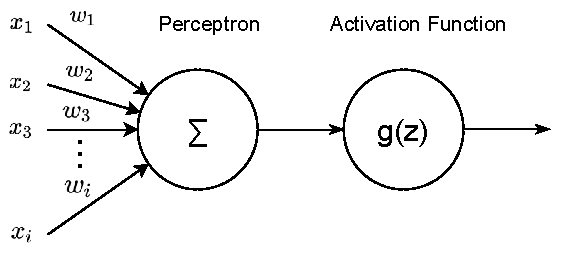
\includegraphics[scale=1]{figures/activation_function.pdf}
    \caption{The structure of a classical neuron.}
    \label{fig:neuron_structure}
\end{figure}

An ideal activation function is continuous and differentiable, so that we can compute the gradient for training, cf. \cite{goodfellow2016deep}. In addition, the range of the activation function should be suitable, not too large or too small. Otherwise, it will affect the efficiency and stability of the training. Despite some of the limitations mentioned above, there are still a wide variety of activation functions available. We will introduce some of them in the following. For more details we refer to \cite{nwankpa2018activation}\cite{dubey2022activation}.

\textbf{The sigmoid function} is given by the relationship

\begin{equation}
    \label{eq:sigmoid}
    \sigma(z)=\frac{1}{1+\exp (-z)}.
\end{equation}

Sigmoid is a classical saturating function. The probability in real life is always limited to the range of 0 to 1, and this characteristic is consistent with the range of sigmoid. Hence, it is common to use sigmoid as activation function when the output is expected to be probabilistic \cite{nwankpa2018activation}. 

\begin{figure}[h!]
    \centering
    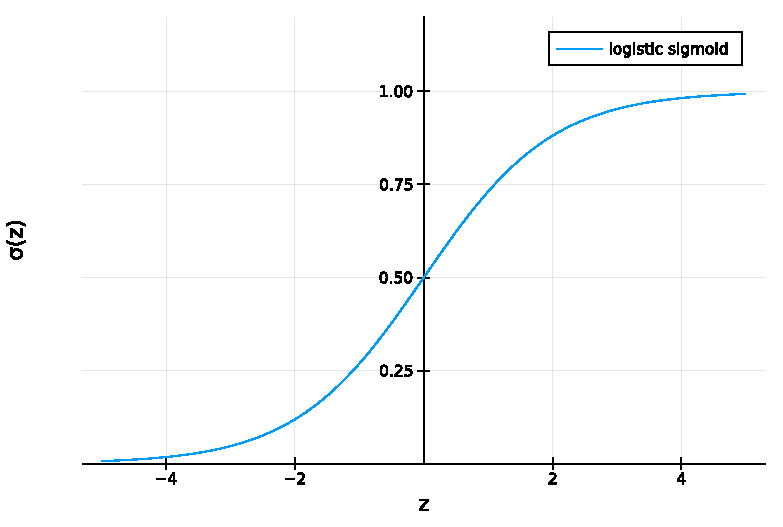
\includegraphics[scale=0.7]{figures/sigmoid.pdf}
    \caption{Logistic sigmoid.}
    \label{fig:sigmoid}
\end{figure}

\textbf{The hyperbolic tangent function} is known as tanh function, which is given by

\begin{equation}
    \label{eq:tanh}
    f(z)=\frac{\left(e^{z}-e^{-z}\right)}{\left(e^{z}+e^{-z}\right)}.
\end{equation}

Compared to sigmoid, tanh function has the range of -1 to 1:

\begin{figure}[h!]
    \centering
    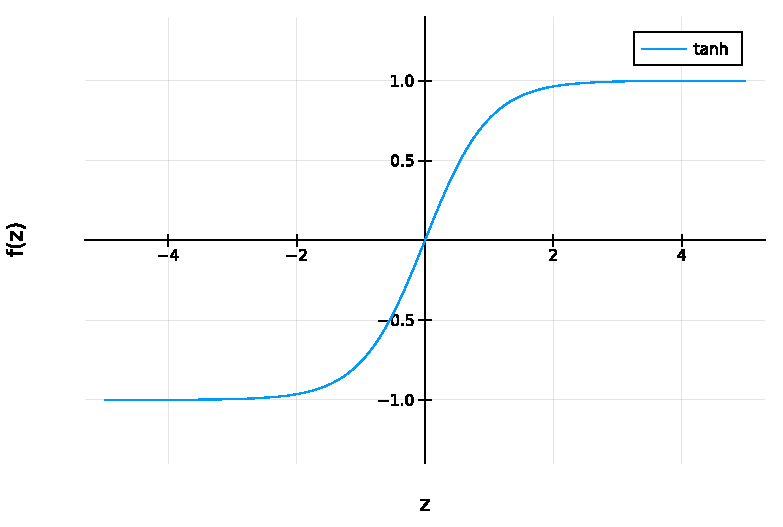
\includegraphics[scale=0.7]{figures/tanh.pdf}
    \caption{Tanh.}
    \label{fig:tanh}
\end{figure}

One characteristic of tanh function is that it is zero-centered, while the sigmoid function is non-zero-centered. The non-zero-centered output is saturated for higher and lower inputs, which leads to vanishing gradient problem. The gradient vanishing problem describes a situation, where the gradient of the objective function with respect to the parameters becomes very close to zero. This situation results in almost no update in the parameters \cite{dubey2022activation}. As a result, the training is almost stopped. In addition, the non-zero-centered characteristic slows down the convergence. Hence, using tanh function as the activation function usually converges faster than using sigmoid function.

\textbf{The Rectified Linear Unit (ReLU) function} is given by the relationship

\begin{equation}
    \label{eq:ReLU}
    ReLU(x) = max(0,x).
\end{equation}

The main advantage of using ReLU is that we only need to perform additions, multiplications and comparison operations, which are more efficient in computation than performing exponentials and divisions \cite{nwankpa2018activation}. However, the ReLU function is still non-zero-centered, which may affect the efficiency of gradient descent. 

\begin{figure}[h!]
    \centering
    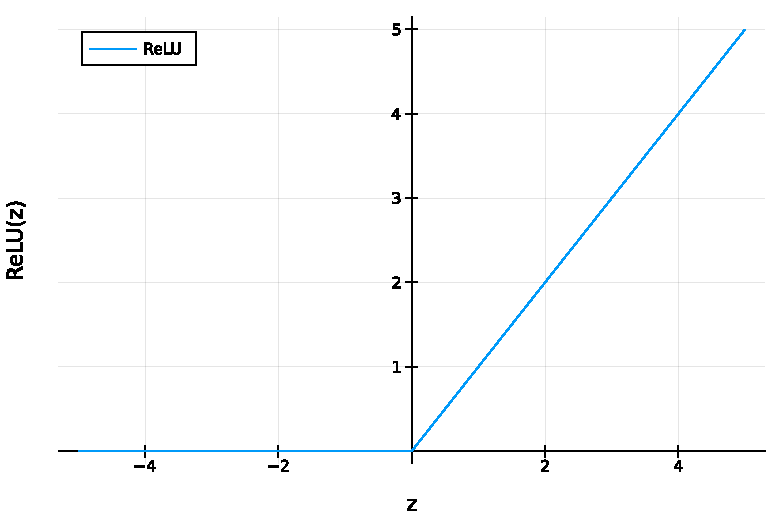
\includegraphics[scale=0.7]{figures/ReLU.pdf}
    \caption{ReLU.}
    \label{fig:ReLU}
\end{figure}


\section{Neural Networks Architectures}
So far, neural networks have evolved a variety of architectures. The following three types of neural network architectures are commonly used: feedforward neural network, feedback neural network and graph neural network.
Take one of the simplest neural network models as an example: a feedforward neural network could be seen as a directed acyclic graph (DAG) with specified input and output nodes, which are fully connected to each other, i.e., the nodes in the later layer are all connected to each node in the former layer. Each node computes its input from the former layer with the parameters and activation function and passes the result to the nodes in the latter layer as their inputs. By definition of a directed acyclic graph, these nodes will never form a closed loop. Figure \ref{fig:feedforward} is an example of feedforward neural network.

\begin{figure}[h!]
    \centering
    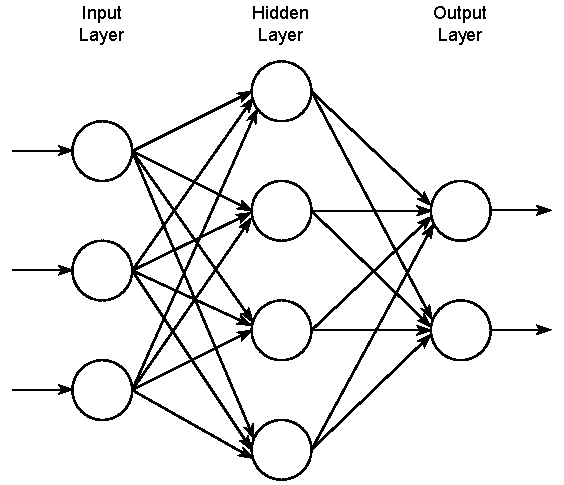
\includegraphics[scale=1]{figures/feedforward_neural_network.pdf}
    \caption{Architecture of a feedforward neural network.}
    \label{fig:feedforward}
\end{figure}

To clarify the principle of feedforward neural network, there are some notations to declare first. The uppercase $L$ stands for the number of total layers (input layer not included) in the feedforward neural network, the lowercase $l$ for the $l$th layer and $M_{l}$ for the number of neurons in $l$th layer. Corresponding to equation \ref{eq:activation_function}, $g_{l}(z^{(l)})$ denotes the activation function in $l$th layer, where $z^{l} \in \mathbb{R}^{M_{l}}$. The parameters weight and bias are represented by the weight matrix $\mathbf{W}^{(l)} \in \mathbb{R}^{M_{l} \times M_{l-1}}$ and the bias vector $\mathbf{b}^{(l)} \in \mathbb{R}^{M_{l}}$. Thus, the input $\mathbf{z}^{(l)}$ and output $\mathbf{a}^{(l)}$ of a neuron in $l$th layer could be written as:

\begin{equation}
    \label{eq:input_output_neuron}
    \begin{aligned}
    \mathbf{z}^{(l)} &= \mathbf{W}^{(l)} \mathbf{a}^{(l-1)} + \mathbf{b}^{(l)}, \quad \mathbf{z}^{(l)} \in \mathbb{R}^{M_{l}}\\
    \mathbf{a}^{(l)} &= g_{l}(\mathbf{z}^{(l)}), \quad \mathbf{a}^{(l)} \in \mathbb{R}^{M_{l}}.
    \end{aligned}
\end{equation}

In fact, the whole feedforward neural network can be seen as a function $f(\mathbf{x};\mathbf{\theta})$, where $\mathbf{x}$ is the input of the neural network and $\mathbf{\theta}$ is the set of the parameters (including weight and bias). Note that the input $\mathbf{x}$ here is the output of the neurons in the input layer, i.e., $\mathbf{x}=[x_1, ..., x_n]=\mathbf{a}^{(0)}$ and the function itself is the output of the neurons in the ouput layer, i.e., $f(\mathbf{x};\mathbf{\theta})=\mathbf{a}^{(L)}$. In general, one can use the feedforward propagation algorithm as the first step to yield initial output to compute the loss function for further optimization. The following is the algorithmic procedure for feedforward propagation:

\clearpage
\begin{algorithm}[h!]
\caption{The feedforward propagation algorithm.}
\label{alg:feedforward_alg}
    \begin{algorithmic}[1]
    \Require neural network $f(\mathbf{x};\mathbf{W},\mathbf{b})$ with $l$th layer
    \Require weight matrix $\mathbf{W} \in \mathbb{R}^{M_{l} \times M_{l-1}}$, bias vector $\mathbf{b} \in \mathbb{R}^{M_{l}}$
    \Require activation function $g(z)$
    \Require input $\mathbf{x}$
    \State $\mathbf{a}^{(0)}=\mathbf{x}$ \Comment{The output of the input layer}
    \For{$l=1...L$}
        \State $\mathbf{z}^{(l)} \gets \mathbf{W}^{(l)} \mathbf{a}^{(l-1)} + \mathbf{b}^{(l)}$ \Comment{Compute the input of a neuron in $l$th layer}
        \State $\mathbf{a}^{(l)} \gets g_{l}(\mathbf{z}^{(l)})$  \Comment{Compute the output of a neuron in $l$th layer}
        \State \Comment{See Equation \ref{eq:input_output_neuron}}
    \EndFor
    \State \Return $f(\mathbf{x};\mathbf{W},\mathbf{b})=\mathbf{a}^{(L)}$ \Comment{Return the initial output}
    \end{algorithmic}
\end{algorithm}

We inplement the feedforward progagation in code:

\begin{minted}[breaklines,escapeinside=||,mathescape=true, linenos, numbersep=3pt, gobble=2, frame=lines, fontsize=\small, framesep=2mm]{julia}
    # 3 neurons in this layer and 2 neurons in the next layer, generate random parameters
    W1 = rand(2, 3)
    b1 = rand(2)
    # 2 neurons in this layer and 4 neurons in the next layer, generate random parameters
    W2 = rand(4, 2)
    b2 = rand(4)
    
    # Input
    a1 = rand(3)
    # The first layer
    z2 = (W1 * a1) .+ b1
    a2 = sigmoid(z2)
    # The second layer
    z3 = (W2 * a2) .+ b2
    a3 = sigmoid(z3)

\end{minted}

\section{Optimization}
An optimization algorithm is ordinarily an algorithm that seeks the optimum. In general, finding the global optimum on a convex objective function is the simplest problem. However, if the objective function is unfortunately a non-convex function, then one has to settle for second best, i.e., seeking the local optimum.

\subsection{Data Set}
A set of samples (or data) is called a data set. In machine learning, there are two types of data set: training set and test set. The training set is used to train the model, while the test set is used to evaluate the model. Such a data set (whether for training or for testing) can be denoted by $\mathcal{D}=\{ (\mathbf{x}_{n}, \mathbf{y}_{n}) \}_{n=1}^{N} = \{ (\mathbf{x}_{1}, \mathbf{y}_{1}),  (\mathbf{x}_{2}, \mathbf{y}_{2}), ..., (\mathbf{x}_{N}, \mathbf{y}_{N}) \}$.

\subsection{Loss Functions}
The loss function $\mathcal{L}\left( y,f(\mathbf{x};\mathbf{\theta}) \right)$ is a non-negative real-valued function that quantifies the error between the target function $y$ and the model prediction $f(\mathbf{x};\mathbf{\theta})$. The following are three common loss functions: zero-one loss function, absolute error loss function and squared error loss function.

Zero-one loss function:

\begin{equation}
    \label{eq:zero_one_loss}
    \mathcal{L}_{0/1}\left( y,f \left(\mathbf{x};\mathbf{\theta} \right) \right) = \begin{cases} 0 & \text{if } y=f(\mathbf{x};\mathbf{\theta}) \\ 1 & \text{if } y \neq f(\mathbf{x};\mathbf{\theta})
    \end{cases}
\end{equation}

The zero-one loss function is pretty intuitive for judging whether the result is good or bad. However, the binary output does not provide some room for further optimization.

Absolute error loss function, also called $\mathcal{L}_{1}$ loss:

\begin{equation}
    \label{eq:AE_loss}
    \mathcal{L}_{1}\left( y,f(\mathbf{x};\mathbf{\theta}) \right) = |y-f(\mathbf{x};\mathbf{\theta})|
\end{equation}

Squared error loss function, also called $\mathcal{L}_{2}$ loss:

\begin{equation}
    \label{eq:SE_loss}
    \mathcal{L}_{2}\left( y,f(\mathbf{x};\mathbf{\theta}) \right) = (y-f(\mathbf{x};\mathbf{\theta}))^2
\end{equation}

The $\mathcal{L}_{1}$ and $\mathcal{L}_{2}$ loss are widely used in linear regression models to evaluate the error. In general, the $\mathcal{L}_{2}$ loss is preferred since it is more sensitive. Yet the $\mathcal{L}_{1}$ loss performs better than the $\mathcal{L}_{2}$ loss in terms of robustness, especially when there are some outliers in the data.

In addition to the mentioned loss function, it is worth noting one concept in statistics: the mean squared error (MSE). In machine learning, MSE is commonly used as the target function for the optimization:

\begin{equation}
    \label{eq:MSE}
    MSE = \frac{1}{N} \sum\nolimits_{n=1}^N \mathcal{L}_{2}\left( y_n,f(\mathbf{x}_n;\mathbf{\theta}) \right) = \frac{1}{N} \sum\nolimits_{n=1}^N (y_n-f(\mathbf{x}_n;\mathbf{\theta}))^2.
\end{equation}


\subsection{Gradient Descent}
Gradient Descent (GD) is the most usual optimization algorithm in machine learning. The idea is to iterate the following procedure:

\begin{equation}
    \label{eq:GD}
    \theta_{t+1} = \theta_{t} - \alpha \frac{1}{N} \sum\nolimits_{n=1}^N \nabla \mathcal{L}\left( y_{n},f(\mathbf{x_{n}};\mathbf{\theta}) \right)
\end{equation}

where $\theta_{t}$ is the parameters at the time step $t$, $\alpha$ is the learning rate and $\nabla \mathcal{L}\left( y^{(n)},f(\mathbf{x^{(n)}};\mathbf{\theta}) \right)$ is the gradient of the loss function:

\begin{equation}
    \label{eq:Gradient_loss}
    \nabla \mathcal{L}\left( y_{n},f(\mathbf{x_{n}};\mathbf{\theta}) \right) = \frac{\partial \mathcal{L}\left( y_{n},f(\mathbf{x_{n}};\mathbf{\theta}) \right)}{\partial \theta}
\end{equation}

The parameters $\theta_{t}$ in each iteration are implemented to the neural network model, and the error (e.g. the mean squared error in Equation \ref{eq:MSE}) is also updated simultaneously with the update of the neural network model. Once the error is small enough to be a desirable value, then the model is considered to be well trained.

\subsection{Stochastic Gradient Descent}
In the gradient descent \ref{eq:GD} above, the target function is the MSE \ref{eq:MSE} over the whole training set, and this approach is called Batch Gradient Descent (BGD).  The Batch Gradient Descent algorithm requires computing the gradient of the loss function for each samples in each iteration. When the size of the training set is large, the space complexity is high and the computational overhead of each iteration is also large.

In order to reduce the computational complexity, it is also possible to pick only one sample in each iteration, compute the gradient of the loss function for this sample and update the parameters. This approach is known as Stochastic Gradient Descent (SGD). For the optimization problems involving non-convex objective function, due to adding the stochastic feature, the SGD algorithm may escape from local optima easier and converge faster than BGD.

\subsection{Backpropagation}
Backpropagation is an algorithm for efficient computation of gradients. The kernel of this algorithm lies in the computation of the partial derivatives of the loss function with respect to parameters, i.e., the gradient in Equation \ref{eq:Gradient_loss}. Since this computation requires the help of automatic differentiation techniques to improve computational efficiency, backpropagation is also known as reverse mode automatic differentiation \cite{baydin2018automatic}.

Consider a neural network $f(\mathbf{x};\mathbf{\theta})=f(\mathbf{x};\mathbf{W},\mathbf{b})$. Based on the chain rule, the partial derivatives of the loss function could be written as the form:

\begin{equation}
    \label{eq:Chain_rule_partial}
    \begin{aligned}
        \frac{\partial \mathcal{L}\left( y,f(\mathbf{x};\mathbf{\mathbf{W},\mathbf{b}}) \right)}{\partial \mathbf{W}^{(l)}} &= \frac{\partial \mathcal{L}\left( y,f(\mathbf{x};\mathbf{\mathbf{W},\mathbf{b}}) \right)}{\partial \mathbf{z}^{(l)}} 
        \frac{\partial \mathbf{z}^{(l)}}{\partial \mathbf{W}^{(l)}}
        \\
        \frac{\partial \mathcal{L}\left( y,f(\mathbf{x};\mathbf{\mathbf{W},\mathbf{b}}) \right)}{\partial \mathbf{b}^{(l)}} &= \frac{\partial \mathcal{L}\left( y,f(\mathbf{x};\mathbf{\mathbf{W},\mathbf{b}}) \right)}{\partial \mathbf{z}^{(l)}}
        \frac{\partial \mathbf{z}^{(l)}}{\partial \mathbf{b}^{(l)}}
    \end{aligned}
\end{equation}

where $\mathbf{z}^{(l)}$ is the input of a neuron in $l$th layer, which is already mentioned above in Equation \ref{eq:input_output_neuron}, i.e., $\mathbf{z}^{(l)} = \mathbf{W}^{(l)} \mathbf{a}^{(l-1)} + \mathbf{b}^{(l)}$. Notice that in Equation \ref{eq:Chain_rule_partial} only three terms to be computed: $\frac{\partial \mathbf{z}^{(l)}}{\partial \mathbf{W}^{(l)}}$, $\frac{\partial \mathbf{z}^{(l)}}{\partial \mathbf{b}^{(l)}}$ and $\frac{\partial \mathcal{L}\left( y,f(\mathbf{x};\mathbf{\mathbf{W},\mathbf{b}}) \right)}{\partial \mathbf{z}^{(l)}}$.

The first two terms are relatively simple to deduce:

\begin{equation}
    \label{eq:two_terms}
    \begin{aligned}
        \frac{\partial \mathbf{z}^{(l)}}{\partial \mathbf{W}^{(l)}} &= \mathbf{a}^{(l-1)}
        \\
        \frac{\partial \mathbf{z}^{(l)}}{\partial \mathbf{b}^{(l)}} &= \mathbf{I},
    \end{aligned}
\end{equation}

where $\mathbf{I}$ is an identity matrix. The third term is called the error, which reflects the sensitivity of the loss to neurons in $l$th layer. It is denoted by $\delta^{(l)}$. Applying the chain rule, the error $\delta^{(l)}$ in terms of the error in the
later layer $\delta^{(l+1)}$ can be written as:

\begin{equation}
    \label{eq:error_in_one_layer}
    \begin{aligned}
        \delta^{(l)} &= \frac{\partial \mathcal{L}\left( y,f(\mathbf{x};\mathbf{\mathbf{W},\mathbf{b}}) \right)}{\partial \mathbf{z}^{(l)}}
        \\
        &= \frac{\partial \mathcal{L}\left( y,f(\mathbf{x};\mathbf{\mathbf{W},\mathbf{b}}) \right)}{\partial \mathbf{z}^{(l+1)}} \cdot \frac{\partial \mathbf{z}^{(l+1)}}{\partial \mathbf{a}^{(l)}} \cdot \frac{\partial \mathbf{a}^{(l)}}{\partial \mathbf{z}^{(l)}}
        \\
        &= (\mathbf{W}^{(l+1)})^T \delta^{(l+1)} \odot g_{l}'(\mathbf{z}^{(l)}),
    \end{aligned}
\end{equation}

where $\mathbf{z}^{(l+1)} = \mathbf{W}^{(l+1)} \mathbf{a}^{(l)} + \mathbf{b}^{(l+1)}$, $\mathbf{a}^{(l)} = g_{l}(\mathbf{z}^{(l)})$ from Equation \ref{eq:input_output_neuron} are plugged into the second line in \ref{eq:error_in_one_layer} and the operation $\odot$ stands for Hadamard product.

After the above deduction, Equation \ref{eq:Chain_rule_partial} together with \ref{eq:two_terms} and \ref{eq:error_in_one_layer} are rewritten in the following form:

\begin{equation}
    \label{eq:Chain_rule_partial_deducted}
    \begin{aligned}
        \frac{\partial \mathcal{L}\left( y,f(\mathbf{x};\mathbf{\mathbf{W},\mathbf{b}}) \right)}{\partial \mathbf{W}^{(l)}} &= \delta^{(l)} (\mathbf{a}^{(l-1)})^T \quad \in \mathbb{R}^{M_{l} \times M_{l-1}}
        \\
        \frac{\partial \mathcal{L}\left( y,f(\mathbf{x};\mathbf{\mathbf{W},\mathbf{b}}) \right)}{\partial \mathbf{b}^{(l)}} &= \delta^{(l)} \quad \in \mathbb{R}^{M_{l}}.
    \end{aligned}
\end{equation}

The algorithm \ref{alg:BP_alg} presents the gradient descent training procedure through backpropagation.

\clearpage
\begin{algorithm}[h!]
\caption{Backpropagation in Stochastic Gradient Descent.}
The backpropagation algorithm requires initial parameters $\theta_{0}$, which is computed by the feedforward propagation algorithm \ref{alg:feedforward_alg}.
\label{alg:BP_alg}
    \begin{algorithmic}[1]
    \Require neural network $f(\mathbf{x};\mathbf{W},\mathbf{b})$ with $l$th layer
    \Require training set $\mathcal{D}=\{(\mathbf{x}_{n}, \mathbf{y}_{n})\}_{N}^{n=1}$
    \Require weight matrix $\mathbf{W} \in \mathbb{R}^{M_{l} \times M_{l-1}}$, bias vector $\mathbf{b} \in \mathbb{R}^{M_{l}}$, initial parameters $\theta_{0}$
    \Require activation function $g(z)$
    \Require regularization parameter $\lambda$
    \Require learning rate $\alpha$

    \For{$l=1...L$}
        \State $\mathbf{z}^{(l)} = \mathbf{W}^{(l)} \mathbf{a}^{(l-1)} + \mathbf{b}^{(l)}$ \Comment{Compute the input of neurons in the $l$th layer}
        \State $\mathbf{a}^{(l)} = g_{l}(\mathbf{z}^{(l)})$ \Comment{Compute the output of neurons in the $l$th layer}
        \State \Comment{See Equation \ref{eq:input_output_neuron}}
        \State $\delta^{(l)} = (\mathbf{W}^{(l+1)})^T \delta^{(l+1)} \odot g_{l}'(\mathbf{z}^{(l)})$ \Comment{Compute the error in the $l$th layer}
        \State \Comment{See Equation \ref{eq:error_in_one_layer}}
        \State $\frac{\partial \mathcal{L}\left( y_n,f(\mathbf{x};\mathbf{\mathbf{W},\mathbf{b}}) \right)}{\partial \mathbf{W}^{(l)}} = \delta^{(l)} (\mathbf{a}^{(l-1)})^T$ \Comment{Compute the gradient on the weight matrix}
        \State $\frac{\partial \mathcal{L}\left( y_n,f(\mathbf{x};\mathbf{\mathbf{W},\mathbf{b}}) \right)}{\partial \mathbf{b}^{(l)}} = \delta^{(l)}$ \Comment{Compute the gradient on the bias vector}
        \State \Comment{See Equation \ref{eq:Chain_rule_partial_deducted}}
        \State $\mathbf{W}^{(l+1)} \gets  \mathbf{W}^{(l)}-\alpha (\delta^{(l)} (\mathbf{a}^{(l-1)})^T + \lambda \mathbf{W}^{(l)})$ \Comment{Update the weight matrix}
        \State $\mathbf{b}^{(l+1)} \gets  \mathbf{b}^{(l)}-\alpha \delta^{(l)}$ \Comment{Update the bias vector}
        \State \Comment{See Equation \ref{eq:GD}}
    \EndFor
    \State \Return $\mathbf{W}, \mathbf{b}$ \Comment{Return the parameters}
    \end{algorithmic}
\end{algorithm}

We can also inplement this algorithm in Julia code. Firstly, we generate random parameters and perform the feedforward propagation with reference to the code of algorithm \ref{alg:feedforward_alg}(the same functionality as the code line 2 and 3 in \ref{alg:BP_alg}):

\begin{minted}[breaklines,escapeinside=||,mathescape=true, linenos, numbersep=3pt, gobble=2, frame=lines, fontsize=\small, framesep=2mm]{julia}
    W = rand(2, 3)
    b = rand(2)
    
    a1 = rand(3)

    z2 = (W1 * a1) .+ b1
    a2 = sigmoid(z2)
\end{minted}

The loss function to be optimized can be defined by:

\begin{minted}[breaklines,escapeinside=||,mathescape=true, linenos, numbersep=3pt, gobble=2, frame=lines, fontsize=\small, framesep=2mm]{julia}
    # Generate random parameters
    W = rand(2, 3)
    b = rand(2)
    # Perform the feedforward propagation
    predict(x) = sigmoid((W * x) .+ b)
    # Define the loss function
    loss(x, y) = mean(abs2, (predict(x) .- y))
    # Compute the loss
    loss(rand(3), rand(2))
\end{minted}

To optimize the loss function, it is necessary to compute the gradient of the loss with respect to the parameters $\frac{\partial \mathcal{L}\left( y_{n},f(\mathbf{x_{n}};\mathbf{\theta}) \right)}{\partial \theta}$(the same functionality as the code line 5, 7 and 8 in \ref{alg:BP_alg}):

\begin{minted}[breaklines,escapeinside=||,mathescape=true, linenos, numbersep=3pt, gobble=2, frame=lines, fontsize=\small, framesep=2mm]{julia}
    # "Flux" is a deep learning framework in Julia language. The function "params" creates a trainable parameters object.
    θ = Flux.params(W, b)
    # Compute the gradient of the loss. "Zygote" is an automatic differentiation package.
    gs = Zygote.gradient(() -> loss(x, y), θ)
    # Compute the gradient of the loss with respect to the parameters
    gs[θ]
\end{minted}

The last step is to update the parameters(the same functionality as the code line 10 and 11 in \ref{alg:BP_alg}):

\begin{minted}[breaklines,escapeinside=||,mathescape=true, linenos, numbersep=3pt, gobble=2, frame=lines, fontsize=\small, framesep=2mm]{julia}
    # The learning Rate
    α = 0.1
    # Update the parameters with the given learning rate and optimization algorithm
    for θ in (W, b)
        θ .-= α * gs[θ]
    end
\end{minted}

Another alternative is to use the function "Flux.Optimise.update!":

\begin{minted}[breaklines,escapeinside=||,mathescape=true, linenos, numbersep=3pt, gobble=2, frame=lines, fontsize=\small, framesep=2mm]{julia}
    # The optimization algorithm
    opt = Flux.Descent(0.1)
    # Update the parameters with the given learning rate and optimization algorithm
    for θ in (W, b)
        Flux.Optimise.update!(opt, θ, gs[θ])
    end
\end{minted}

As can be seen, backpropagation involves the calculation of gradients in computer programs, and automatic differentiation is a powerful tool in this regard.

\subsection{Automatic Differentiation}
Automatic differentiation (AD) is a set of techniques that allow a computer program to yield the derivative of a function. Automatic differentiation uses the fact that any computer program that implements a vector-valued function could be decomposed into a sequence of basic specified operations, each of which can be easily differentiated by looking up a table. These basic partial derivatives that compute a particular term are combined into a differential form, such as gradient, Jacobian, etc.

\subsection{Adam Algorithm}
As can be seen from the process of backpropagation above, the gradient descent algorithm is actually applied in the step of updating the parameters. So are there any other algorithms to update the parameters besides the gradient descent algorithm? The answer is yes. For example, one can use the momentum method to replace the gradient $\nabla \mathcal{L}(\cdot)$ with momenta and the RMSProp algorithm (Root Mean Squared Propagation algorithm) \cite{tieleman2012divide} to update the learning rate $\alpha$. An algorithms that combines the ideas of the momentum method and the RMSProp algorithm is the Adam algorithms (Adaptive Moment Estimation Algorithm) \cite{kingma2014adam}. In practice, the Adam algorithm shows better performance, i.e., fewer parameters to tune and resulting in higher computational efficiency.

The Adam algorithm uses mini-batch gradient descent \cite{bottou2010large}. Consider a neural network $f(\mathbf{x};\mathbf{W},\mathbf{b})$, a training set $\mathcal{D}=\{ (\mathbf{x}_{n}, \mathbf{y}_{n}) \}_{n=1}^{N}$. Mini-batch gradient descent algorithm splits the training set $\mathcal{D}$ into a sequence of subsets (or mini batches) $\mathcal{S}_t=\{(\mathbf{x}_{m}, \mathbf{y}_{m}) \}_{m=1}^{M}$ for each iteration $t$, where $M$ is the batch size of one of the mini batches.

Similar to the idea of gradient descent (see \ref{eq:GD}), the point of the Adam algorithm is to iterate the following procedure:

\begin{equation}
    \label{eq:Adam_GD}
    \begin{aligned}
        \theta_{t+1} = \theta_{t} - \alpha \frac{\hat{s}}{\sqrt{\hat{r}} + \epsilon},
    \end{aligned}
\end{equation}

where $\epsilon$ is a very small constant for stabilization (avoiding a denominator of zero). And the two terms $\hat{s}$ and $\hat{r}$ are known as correct moment estimate. It corrected the bias of the original moment estimate $s$ and $r$ at the beginning of the iteration:

\begin{equation}
    \label{eq:correct_moment_estimate}
    \begin{aligned}
        \hat{s_t} &= \frac{s_t}{1-\beta_1^t}
        \\
        \hat{r_t} &= \frac{r_t}{1-\beta_2^t},
    \end{aligned}
\end{equation}

where $\beta_1^t$ and $\beta_2^t$ are learning rate decay. The moment estimate $s_t$ and $r_t$ are defined as following:

\begin{equation}
    \label{eq:moment_estimate}
    \begin{aligned}
        s_t &= \beta_1 s_{t-1} + (1-\beta_1) \mathbf{g_t}
        \\
        r_t &= \beta_2 r_{t-1} + (1-\beta_2) \mathbf{g_t} \odot \mathbf{g_t}
    \end{aligned}
\end{equation}

where $\mathbf{g_t}$ stands for the gradient of the loss function with respect to the parameter at $t$th iteration over the mini-batch:

\begin{equation}
    \label{eq:mean_gradient}
    \mathbf{g_t} = \frac{1}{M} \sum\nolimits_{m=1}^M \nabla \mathcal{L}\left( y_{m},f(\mathbf{x};\mathbf{\theta}) \right).
\end{equation}
 

\clearpage
\begin{algorithm}[h!]
\caption{The training procedure of the Adam algorithm.}
The decay rates $\beta_1$ and $\beta_2$ should be within the range of $[0,1)$, f.e., $\beta_1=0.9$ and $\beta_2=0.99$ and the learning rate $\alpha$ is recommended to be 0.001. And the very small constant $\epsilon$ is set to $10^{-8}$.
\label{alg:Adam_alg}
    \begin{algorithmic}[1]
    \Require neural network $f(\mathbf{x};\mathbf{W},\mathbf{b})$ with $l$th layer
    \Require weight matrix $\mathbf{W} \in \mathbb{R}^{M_{l} \times M_{l-1}}$, bias vector $\mathbf{b} \in \mathbb{R}^{M_{l}}$, initial parameters $\theta_{0}$
    \Require activation function $g(z)$
    \Require decay rate $\beta_1$ and $\beta_2$
    \Require learning rate $\alpha$
    \Require constant $\epsilon$
    \For{$m=1...M$} \Comment{Iterate all elements in the current mini-batch}
        \For{$l=1...L$}
            \State $\mathbf{z}^{(l)} = \mathbf{W}^{(l)} \mathbf{a}^{(l-1)} + \mathbf{b}^{(l)}$ \Comment{Compute the input of neurons in the $l$th layer}
            \State $\mathbf{a}^{(l)} = g_{l}(\mathbf{z}^{(l)})$ \Comment{Compute the output of neurons in the $l$th layer}
            \State \Comment{See Equation \ref{eq:input_output_neuron}}
            \State $\delta^{(l)} = (\mathbf{W}^{(l+1)})^T \delta^{(l+1)} \odot g_{l}'(\mathbf{z}^{(l)})$ \Comment{Compute the error in the $l$th layer}
            \State \Comment{See Equation \ref{eq:error_in_one_layer}}
            \State $\frac{\partial \mathcal{L}\left( y_m,f(\mathbf{x};\mathbf{\mathbf{W},\mathbf{b}}) \right)}{\partial \mathbf{W}^{(l)}} = \delta^{(l)} (\mathbf{a}^{(l-1)})^T$ \Comment{Compute the gradient on the weight matrix}
            \State $\frac{\partial \mathcal{L}\left( y_m,f(\mathbf{x};\mathbf{\mathbf{W},\mathbf{b}}) \right)}{\partial \mathbf{b}^{(l)}} = \delta^{(l)}$ \Comment{Compute the gradient on the bias vector}
            \State \Comment{See Equation \ref{eq:Chain_rule_partial_deducted}}
        \EndFor
    \EndFor
    \State $\mathbf{g_t} \gets \frac{1}{M} \sum\nolimits_{m=1}^M \nabla \mathcal{L}\left( y_{m},f(\mathbf{x};\mathbf{\theta}) \right)$ \Comment{Compute the mean gradient, see Equation \ref{eq:mean_gradient}}
    \State $s_t \gets \beta_1 s_{t-1} + (1-\beta_1) \mathbf{g_t}$ \Comment{Compute the fist moment estimate}
    \State $r_t \gets \beta_2 r_{t-1} + (1-\beta_2) \mathbf{g_t} \odot \mathbf{g_t}$ \Comment{Compute the second moment estimate}
    \State \Comment{See Equation \ref{eq:moment_estimate}}
    \State $\hat{s_t} \gets \frac{s_t}{1-\beta_1^t}$ \Comment{Correct the bias}
    \State $\hat{r_t} \gets \frac{r_t}{1-\beta_2^t}$ \Comment{Correct the bias}
    \State \Comment{See Equation \ref{eq:correct_moment_estimate}}
    \State $\theta_{t+1} \gets \theta_{t} - \alpha \frac{\hat{s}}{\sqrt{\hat{r}} + \epsilon}$ \Comment{Update the parameters}
    \State \Comment{See Equation \ref{eq:Adam_GD}}
    \State \Return $\mathbf{W}, \mathbf{b}$ \Comment{Return the parameters}
    \end{algorithmic}
\end{algorithm}

The inplementation of Adam algorithm is similar to the algorithm \ref{alg:BP_alg}. However, the Adam algorithm uses mini-batch gradient descent:

\begin{minted}[breaklines,escapeinside=||,mathescape=true, linenos, numbersep=3pt, gobble=2, frame=lines, fontsize=\small, framesep=2mm]{julia}
    # The ADAM algorithm with the learning rate α=0.01 and decay rates β1=0.9, β2=0.99.
    opt = Flux.Optimise.ADAM(0.01, (0.9, 0.99))
    # Construct a function to compute the gradients
    θ = Flux.params(W, b)
    gs(x, y) = Zygote.gradient(() -> loss(x, y), θ)
    # Construct a dataloader. "dataloader" is an iterable object, which yields a batch of data with the specified batchsize in each iteration. For instance, now we have 1000 points in the training set (x, y). A dataloader with the given batchsize 10 will generate only 10 points in each iteration.
    dataloader = Flux.Data.DataLoader((x, y), batchsize = 10)

    # Update the parameters with the given learning rate and optimization algorithm
    for (x, y) in dataloader
        for θ in (W, b) 
            Flux.Optimise.update!(opt, θ, gs(x, y)[θ])
        end
    end
\end{minted}

\clearpage
\chapter{Neural ODEs}
\label{ch:chapter5}
In order to obtain more accurate results from a neural network model, one may tend to think of stacking more hidden layers. However, when some data scientists try to build complex models using neural networks with hundreds of hidden layers, they found that the vanishing or exploding gradient problem often occurs in backpropagation, which seriously affects the learning efficiency of the upstream hidden layers \cite{glorot2010understanding}. Due to the vanishing or exploding gradient problem, a deeper neural network could even yield worse results than a shallower one. And ResNet (Residual Neural Network) was exactly designed to tackle these problems \cite{he2016deep}. The proposers of ResNet argue that the results of deeper neural networks can be better or at least equal to the results of shallower neural networks, but should not be worse.

\section{Residual Neural Networks}
In the traditional convention, the output of a layer of a neural network can only be given as input to the next neighboring layer of the neural network. The ResNet breaks this traditional convention, i.e., it allows the output of a layer $\mathbf{x}$ to skip several weight layers $F(\mathbf{x};\theta)$ directly. Then, the output $\mathbf{x}$ can be used as the input to a latter layer:

\begin{equation}
    \label{eq:ResNet}
    H(\mathbf{x})=\mathbf{x}+F(\mathbf{x};\theta),
\end{equation}

where $H$ is the output or target function. The residual building block illustrates what equation \ref{eq:ResNet} does:

\clearpage
\begin{figure}[htbp!]
    \centering
    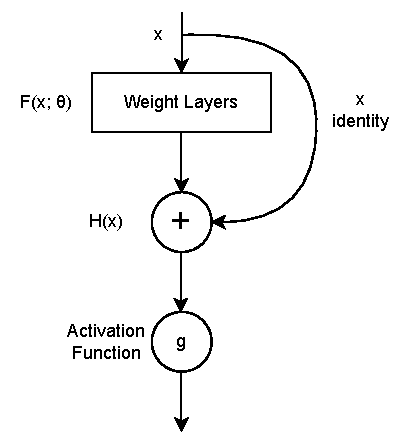
\includegraphics[scale=1]{figures/ResNet.pdf}
    \caption{Residual building block.}
    \label{fig:ResNet}
\end{figure}

The weight layers could be thought of as two or more hidden layers that are skipped over by a shortcut connection. This shortcut connection changes the learning target from learning the complete output $H(\mathbf{x})$ to the residual $H(\mathbf{x})-\mathbf{x}$. And the goal of the optimization is to minimize the residual $H(\mathbf{x})-\mathbf{x}$ and make it close to zero. In this case, if $F(\mathbf{x};\theta)=H(\mathbf{x})-\mathbf{x}=0$, then $H(\mathbf{x})=\mathbf{x}$. Since the output $H(\mathbf{x})$ and the input $\mathbf{x}$ are identical, $\mathbf{x}$ can be called identity. The proposers of ResNet hypothesized that the residual is easier to optimize than the complete output and then verified this hypothesis in their experiments. 

 The significance of ResNet is that it provides a new direction to address the challenges of stacking more and more hidden layers to the neural networks. Benefiting from the ResNet, the vanishing or exploding gradient problem can be solved to some extent.

\section{Neural ODEs}
The hidden layers in a ResNet are built by a sequence of transformations in Equation \ref{eq:ResNet}. This sequence of transformations was found to be remarkably similar to the Euler method \ref{eq:Eulers_method_explicit} \cite{ruthotto2020deep}. In view of this, equation \ref{eq:ResNet} can also be rewritten as

\begin{equation}
    \label{eq:Euler_discretization}
    \mathbf{z}_{t+1} = \mathbf{z}_{t} + f(\mathbf{z}_{t}; \theta),
\end{equation}

where $t \in {0 ... T}$. Such a sequence of iterations is an Euler discretization of a continuous transformation.

Equation \ref{eq:Euler_discretization} can be rewritten in the form:

\begin{equation}
    \label{eq:Euler_discretization_rewritten}
    \frac{\mathbf{z}_{t+1}-\mathbf{z}_{t}}{\Delta t} = f(\mathbf{z}_{t}; \theta),
\end{equation}

where $\Delta t = (t+1)-t = 1$. If $\Delta t$ is a very small step, rewrite \ref{eq:Euler_discretization_rewritten} as

\begin{equation}
    \label{eq:Euler_discretization_small_step}
    \lim_{\Delta t \to 0} \frac{\mathbf{z}_{t+1}-\mathbf{z}_{t}}{\Delta t} = f(\mathbf{z}_{t}; \theta).
\end{equation}

The LHS of \ref{eq:Euler_discretization_small_step} can be considered as the gradient of $z(t)$ by the definition of differentiation, i.e.,

\begin{equation}
    \label{eq:Euler_discretization_differentiation}
    \frac{d\mathbf{z}(t)}{dt} = f(\mathbf{z}(t), t; \theta).
\end{equation}

Plug \ref{eq:Euler_discretization_differentiation} into \ref{eq:Euler_discretization}. An equation such as 

\begin{equation}
    \label{eq:Neural_ODE}
    \mathbf{z}(t+\varepsilon ) = \mathbf{z}(t) + \int_{t}^{t+\varepsilon } f(\mathbf{z}(t), t, \theta)dt
\end{equation}

is called Neural ODE (Neural Ordinary Differential Equation) \cite{chen2018neural}, where $\varepsilon $ is a small time step and the RHS $f(\mathbf{z}(t), t; \theta)$ can be considered as a neural network $NN(\mathbf{z}(t), t; \theta)$. An ODE solver is treated as a black box that provides a solution to the ODE. Thus, the loss function to be optimized is of the form

\begin{equation}
    \label{eq:Neural_ODE_Gradient_loss}
    \begin{aligned}
    \mathcal{L}(\mathbf{z}(t+\varepsilon )) &= \mathcal{L}(\mathbf{z}(t) + \int_{t}^{t+\varepsilon } f(\mathbf{z}(t), t, \theta)dt \:)\\
    &= \mathcal{L}(ODESolver(\mathbf{z}(t), f, t, t+\varepsilon , \theta)).
    \end{aligned}
\end{equation}

To optimize the loss function \ref{eq:Neural_ODE_Gradient_loss} through backpropagation, one needs to compute the gradient of the loss function \ref{eq:Gradient_loss}. The next step, to calculate the error, is to mimic the procedure in Equation \ref{eq:error_in_one_layer}:

\begin{equation}
    \label{eq:Neural_ODE_error}
    \frac{d\mathcal{L}}{d\mathbf{z}(t)} = \frac{d\mathcal{L}}{d\mathbf{z}(t+\varepsilon )} \cdot \frac{d\mathbf{z}(t+\varepsilon )}{d\mathbf{z}(t)}.
\end{equation}

\section{Adjoint Method}
The adjoint method (or adjoint sensitivity method) is a method used to compute the gradients of functions efficiently, which can be dated back to the 1960s \cite{boltyanskiy1962mathematical}. Due to the continuity of Neural ODE, computing the gradient of the loss function in backpropagation leads to a huge memory cost. The significance of using the adjoint method is that the gradient of the loss function can still be computed efficiently without storing the intermediate activations which have a huge memory overhead.

Similar to the algorithm \ref{alg:BP_alg} in the preceding chapter, the goal of the adjoint method is also to compute the gradient of the loss function with respect to the state $\frac{d\mathcal{L}}{d\mathbf{z}(t)}$ and with respect to the parameters $\frac{d\mathcal{L}}{d\theta}$.

To use the adjoint method, the first step is to define an adjoint state that equal to the gradient of the loss function with respect to the state:

\begin{equation}
    \label{eq:adjoint_state}
    \mathbf{a}(t) = \frac{d\mathcal{L}}{d\mathbf{z}(t)}.
\end{equation}

After that, expand the Taylor series for the hidden state $\mathbf{z}(t+\varepsilon )$ at the point $\mathbf{z}(t)$:

\begin{equation}
    \label{eq:taylor_series_expansion}
    \begin{aligned}
    \mathbf{z}(t+\varepsilon ) &= \mathbf{z}(t) + \int_{t}^{t+\varepsilon } f(\mathbf{z}(t), t, \theta)dt\\
    &= \mathbf{z}(t) + \varepsilon f(\mathbf{z}(t), t; \theta) + O (\varepsilon ^2).
    \end{aligned}
\end{equation}

Then plug the equations \ref{eq:adjoint_state} and \ref{eq:taylor_series_expansion} into Equation \ref{eq:Neural_ODE_error}:

\begin{equation}
    \label{eq:Neural_ODE_adjoint_state}
    \mathbf{a}(t) = \mathbf{a}(t+\varepsilon ) \cdot \frac{\partial}{\partial \mathbf{z}(t)} (\mathbf{z}(t) + \varepsilon f(\mathbf{z}(t), t; \theta) + O (\varepsilon ^2)) .
\end{equation}

By the definition of differentiation, the gradient of the adjoint state follows:

\begin{equation}
    \label{eq:adjoint_state_gradient_hidden_state}
    \begin{aligned}
        \frac{d\mathbf{a}(t)}{dt} &= \lim_{\varepsilon \to 0+} \frac{\mathbf{a(t+\varepsilon)}-\mathbf{a(t)}}{\varepsilon} \\
        &= \lim_{\varepsilon \to 0+} \frac{\mathbf{a(t+\varepsilon)}-\mathbf{a}(t+\varepsilon ) \cdot \frac{\partial}{\partial \mathbf{z}(t)} (\mathbf{z}(t) + \varepsilon f(\mathbf{z}(t), t; \theta) + O (\varepsilon ^2)) }{\varepsilon}\\
        &= \lim_{\varepsilon \to 0+} \frac{-\varepsilon \mathbf{a(t+\varepsilon)} \frac{\partial f(\mathbf{z}(t), t; \theta)}{\partial \mathbf{z}(t)} + O (\varepsilon ^2)}{\varepsilon}\\
        &= \lim_{\varepsilon \to 0+} - \mathbf{a(t+\varepsilon)} \frac{\partial f(\mathbf{z}(t), t; \theta)}{\partial \mathbf{z}(t)} + O (\varepsilon)\\
        &= - \mathbf{a(t)} \frac{\partial f(\mathbf{z}(t), t; \theta)}{\partial \mathbf{z}(t)}
    \end{aligned}
\end{equation}

Now perform the feedforward propagation algorithm \ref{alg:feedforward_alg}  to get the initial output and compute the initial adjoint state $\mathbf{a}(T) = \frac{d\mathcal{L}}{d\mathbf{z}(T)}$ with reference to Equation \ref{eq:adjoint_state}. This can be considered as the initial condition of an ODE problem. And the corresponding ODE is of the form:

\begin{equation}
    \label{eq:adjoint_state_ODE}
    \begin{aligned}
    \mathbf{a}(T-\varepsilon) &= \mathbf{a}(T) + \int_{T}^{T-\varepsilon} \frac{d\mathbf{a(t)}}{dt} \\
    &= \mathbf{a}(T) - \int_{T}^{T-\varepsilon} \mathbf{a(t)}^T \frac{\partial f(\mathbf{z}(t), t; \theta)}{\partial \mathbf{z}(t)} \quad \text{plugging} \: \ref{eq:adjoint_state_gradient_hidden_state} \\ 
    \end{aligned}
\end{equation}

Note that the adjoint state $\mathbf{a(t)}^T$ is transposed due to the "backward" direction.

Similar to Equation \ref{eq:adjoint_state} $\mathbf{a}(t) = \frac{d\mathcal{L}}{d\mathbf{z}(t)}$, the gradient of the loss function with respect to the parameters is defined by:

\begin{equation}
    \label{eq:adjoint_state_parameters}
    \mathbf{a_\theta}(t) = \frac{d\mathcal{L}}{d\theta}.
\end{equation}

The corresponding gradient of the adjoint state is of the form:

\begin{equation}
    \label{eq:adjoint_state_gradient_parameters}
    \frac{d\mathcal{L}}{d\theta} = - \int_{T}^{0} \mathbf{a(t)}^T \frac{\partial f(\mathbf{z}(t), t; \theta)}{\partial \mathbf{\theta}} dt
\end{equation}


More details for $\frac{d\mathcal{L}}{d\theta}$ can be found in the original paper \cite{chen2018neural}.

A short summary: From the above procedures, it can be concluded that the idea of the adjoint method in Neural ODE is to compute a sequence of adjoint states in a "backward" direction by solving ODEs, and therefore the gradients can also be computed in an indirect manner.


\clearpage
\chapter{Structured ODE Neural Networks}
\label{ch:chapter6}
\section{Physics Priors}
In machine learning, some optimization algorithms tend to make some assumptions to improve the learning efficiency, and these assumptions are called inductive biases (also known as priors) \cite{mitchell1997machine}. Inductive biases or priors may have different names in specific fields. For example, in the field of physics, they are most frequently referred to as physics priors or physically informed inductive biases.

The experiments in \cite{gupta2019general} introduced a framework to model the Lagrangian and the generalized forces of mechanical systems by using neural networks. Their experiments show the advantage of a gray-box model endowed with physics priors in terms of data efficiency compared to a black-box model without prior knowledge. Another similar work related to Lagrangian is \cite{lutter2019deep}.

In the field of Hamiltonian systems, \cite{greydanus2019hamiltonian} proposed an approach to learn a parametric Hamiltonian function $H_{\theta}$ from the time derivatives of coordinates in the way that $\frac{\partial \mathcal{H}_{\theta}}{\partial \mathbf{p}} - \frac{d\mathbf{q}}{dt} = 0, \frac{\partial \mathcal{H}_{\theta}}{\partial \mathbf{q}} - \frac{d\mathbf{p}}{dt} = 0 $. Such an approach allows HNNs (Hamiltonian Neural Networks) to learn a conserved quantity that is analogous to the total energy.

\section{Neural Networks for Learning of Hamiltonian Systems}
In \cite{chen2019symplectic}, they compared two neural network models of Hamiltonian systems: O-NETs (ODE Neural Networks) and H-NETs (Hamiltonian Neural Networks), where H-NETs follow the idea of HNNs. 
Before introducing O-NETs and H-NETs, recall that a Neural ODE \ref{eq:Neural_ODE} contains a neural network $f$. An ODE solver provides a solution to the ODE such that $\mathbf{z}(t+\varepsilon) = ODESolver(\mathbf{z}(t), f, t, t+\varepsilon , \theta)$. Note that in \cite{chen2019symplectic}, $f$ is considered as a neural network (e.g. in the case of O-NETs). However, $f$ can also be a function that contains a neural network (e.g. in the case of HNNs or H-NETs). 

For better understanding, We will use Julia code to explain the central ideas of O-NET and H-NET in the following.

\subsection{O-NETs}
O-NET is a neural network in a Neural ODE, which can be denoted by $f_{\theta}$. The training of an O-NET can be conceptually divided into five steps.

\textbf{Step 1}: construct a neural network

 We can construct a 2-input and 2-output O-NET via the deep learning framework Flux.jl or Lux.jl.
\begin{minted}[breaklines,escapeinside=||,mathescape=true, linenos, numbersep=3pt, gobble=2, frame=lines, fontsize=\small, framesep=2mm]{julia}
    # Dense: construct a layer. For instance, Dense(2, 40, tanh) constructs a 2-input and 40-output layer with the activation function tanh.
    # Chain: connect layers.
    # O_NET: a feedforward neural network with 2 neurons in the input layer, 40 neurons in the first hidden layer, 40 neurons in the second hidden layer and 2 neurons in the output layer.

    O_NET = Chain(Dense(2, 40, tanh),
                  Dense(40, 40, tanh),
                  Dense(40, 2))
\end{minted}

If we use both Flux.jl and Lux.jl simultaneously (sometimes a mix of both may be needed), then it is advisable to specify them explicitly, as they both contain chain and dense functions under the same name. However, the ways of generating initial parameters and obtaining output are different in both.

In Flux:
\begin{minted}[breaklines,escapeinside=||,mathescape=true, linenos, numbersep=3pt, gobble=2, frame=lines, fontsize=\small, framesep=2mm]{julia}
    O_NET = Flux.Chain(Flux.Dense(2, 40, tanh),
                       Flux.Dense(40, 40, tanh),
                       Flux.Dense(40, 2))
    # ps: the initial parameters of the neural network. 
    # re: a method to reconstruct the neural network with the given parameters ps and input x, e.g., re(ps)(x) is the output of the neural network with the given parameters ps and input x.
    ps, re = Flux.destructure(O_NET)
\end{minted}

In Lux:
\begin{minted}[breaklines,escapeinside=||,mathescape=true, linenos, numbersep=3pt, gobble=2, frame=lines, fontsize=\small, framesep=2mm]{julia}
    O_NET = Lux.Chain(Lux.Dense(2, 40, tanh),
                      Lux.Dense(40, 40, tanh),
                      Lux.Dense(40, 2))
    # "Random.default_rng" is a random number generator. It generates a random number in preparation for generating random parameters in the next code line.
    using Random
    rng = Random.default_rng()
    # ps: the initial parameters of the neural network.
    # st: the state of the neural network. It stores information (layers number, neurons number, activation function etc.) for reconstructing the neural network. For example, the output of the neural network with the given parameters is O_NET(x, ps, st)
    ps, st = Lux.setup(rng, O_NET)
\end{minted}

\textbf{Step 2}: construct an IVP

Suppose that $\{ \mathbf{z}_{t} \}_{t=1}^{T}$ is a training set, where $\mathbf{z}_{t}$ are some discrete points from a trajectory observation. Given an initial state $\mathbf{z}_{0}$ and time steps $\{ t \}_{t=0}^{T}$, we define an IVP

\begin{equation}
    \label{eq:O-NET_IVP}
    \dot{\mathbf{z}}_t = f_{\theta}(\mathbf{z_t}) = NN(\mathbf{z_t}, \theta), \quad \mathbf{z}(t_{0}) = \mathbf{z}_{0},
\end{equation}

where $NN$ is an O-NET.

$f_{\theta}(\mathbf{z_t})$ at the fixed time $t$ estimates the time derivative of coordinates $\dot{\mathbf{z}}_{t}$ such that $\dot{ \mathbf{z}}_{t} = f_{\theta}(\mathbf{z}_t)$. In the case of Hamiltonian systems, let $\mathbf{z}_{t} = [q_{t}, p_{t}]$, we can rewrite the IVP \ref{eq:O-NET_IVP} as $[\dot q_{t}, \dot p_{t}] = f_{\theta}(q_t, p_t) = \text{NN}(\mathbf{z_t}, \theta)$, $\mathbf{z}_{0}= [q_{0}, p_{0}]$.

Let $\mathbf{z}_{0}=[1.0, 1.0]$ and $\{ t \}_{t=0}^{19.9} = (0.0, 0.1, 19.9)$, we construct this IVP in code:

\begin{minted}[breaklines,escapeinside=||,mathescape=true, linenos, numbersep=3pt, gobble=2, frame=lines, fontsize=\small, framesep=2mm]{julia}
    # dz is the time derivative of z at a fixed time.
    # Note: the "t" in the argument is designed for nonautonomous case. This "t" is not the same concept as timesteps. In the case of Hamiltonian (autonomous), this "t" will not be used.
    function ODE(dz, z, θ, t)
    # In Flux.jl, re(θ)(z) is the output of O-NET with the given parameters θ and input z. In Lux.jl, this term should be rewritten as O_NET(z, θ, st).
    dz[1] = re(θ)(z)[1]
    dz[2] = re(θ)(z)[2]
    end
    
    initial_state = [1.0, 1.0]
    
    # Starting at 0.0 and ending at 19.9, the length of each single step is 0.1. Thus, we have 200 time steps in total.
    time_span = (0.0, 19.9)
    time_steps = range(0.0, 19.9, 200)
    
    θ = ps
    
    # ODEProblem is an IVP constructor in the Julia package SciMLBase.jl
    using SciMLBase
    IVP = SciMLBase.ODEProblem(ODEFunction(ODE), initial_state, time_span, θ)
\end{minted}

\textbf{Step 3}: solve the IVP

To obtain the estimate of the coordinates trajectories $q_t$ and $p_t$, we can use an ODE solver to yield the solution of the IVP \ref{eq:O-NET_IVP}

\begin{equation}
    \label{eq:O-NET_ODESolver}
    \{ \hat{z_{t}} \}_{t=1}^{T} = ODESolver(z_{0}, f_{\theta}, \{ t \}_{t=1}^{T}).
\end{equation}

To solve the IVP \ref{eq:O-NET_IVP} in Julia code, we use the package CommonSolve.jl, which provides a common interface for distinct ODE solvers:

\begin{minted}[breaklines,escapeinside=||,mathescape=true, linenos, numbersep=3pt, gobble=2, frame=lines, fontsize=\small, framesep=2mm]{julia}
    # Select a numerical method to solve the IVP
    using OrdinaryDiffEq
    numerical_method = ImplicitMidpoint()
    
    # Select the adjoint method to computer the gradient of the loss with respect to the parameters. ReverseDiffVJP is a callable function in the package SciMLSensitivity.jl, it uses the automatic differentiation tool ReverseDiff.jl to compute the vector-Jacobian products (VJP) efficiently. For more details about adjoint method, please refer to the Neural ODE chapter.
    using SciMLSensitivity
    sensitivity_analysis = InterpolatingAdjoint(autojacvec=ReverseDiffVJP(true))
    
    # Use the ODE Solver CommonSolve.solve to yield solution. And the solution is the estimate of the coordinates trajectories.
    using CommonSolve
    solution = CommonSolve.solve(IVP, numerical_method, p=θ, tstops = time_steps, sensealg=sensitivity_analysis)
    
    # Convert the solution into a 2D-array
    pred_data = Array(solution)
\end{minted}

The final variable "pred\_data" is a 2D-array, which stands for the estimate of the coordinates trajectories $\{ \hat{z_{t}} \}_{t=1}^{T}$. In our case, we have 2 coordinates (q, p) in the Hamiltonian system and 200 time steps. Thus, the "pred\_data" is a $2 \times 200$ array.

\textbf{Step 4}: construct a loss function

To train the neural network model, we define a loss function

\begin{equation}
    \label{eq:loss_O-NET}
    \mathcal{L} = \lVert \mathbf{z}_{t} - \hat{\mathbf{z}_{t}} \rVert_{2},
\end{equation}

where $\hat{\mathbf{z}_{t}}$ is the estimate at a fixed time $t$ ($\hat{\mathbf{z}_{t}}$ is a point in the estimate of the coordinates trajectories $\{ \hat{z_{t}} \}_{t=1}^{T}$) and $\mathbf{z}_{t}$ is assumed to be a point from observation (${\mathbf{z}_{t}}$ is a point in the training set $\{ {z_{t}} \}_{t=1}^{T}$). The goal of the optimization is to minimize the error between them.

However, in code, we adopt the training set $\{ {z_{t}} \}_{t=1}^{T}$ generated by the system of ODEs instead of real observations. For instance, the training set for an undamped harmonic oscillator can be generated by the system of ODEs \ref{eq:ODE_undamped_harmonic_oscillator}:

\begin{minted}[breaklines,escapeinside=||,mathescape=true, linenos, numbersep=3pt, gobble=2, frame=lines, fontsize=\small, framesep=2mm]{julia}
    # The system of ODEs of an undamped harmonic oscillator
    function ODEfunc_udho(dz, z, params, t)
      q, p = z
      m, c = params
      dz[1] = p/m
      dz[2] = -q/c
    end
    # params = [m, c]
    params = [2, 1] 
    prob = ODEProblem(ODEFunction(ODEfunc_udho), initial_state, time_span, params)
    ode_data = Array(CommonSolve.solve(prob, ImplicitMidpoint(), tstops = time_steps))
\end{minted}

The "ode\_data" can be expressed by $\{ z_{t} \}_{t=1}^{T}$. The loss function \ref{eq:loss_O-NET} is the squared difference between a point in "pred\_data" $\{ \hat{z_{t}} \}_{t=1}^{T}$ and a point in "ode\_data" $\{ z_{t} \}_{t=1}^{T}$ at a fixed time $t$.

Now we can construct the loss function in code:
\begin{minted}[breaklines,escapeinside=||,mathescape=true, linenos, numbersep=3pt, gobble=2, frame=lines, fontsize=\small, framesep=2mm]{julia}
function solve_IVP(θ, batch_timesteps)
    IVP = SciMLBase.ODEProblem(ODEFunction(ODE), initial_state, (batch_timesteps[1], batch_timesteps[end]), θ)
    pred_data = Array(CommonSolve.solve(IVP, Midpoint(), p=θ, saveat = batch_timesteps, sensealg=sensitivity_analysis))
    return pred_data
end

function loss_function(θ, batch_data, batch_timesteps)
    pred_data, _ = solve_IVP(θ, batch_timesteps)
    # "batch_data" is a batch of ode data
    loss = sum((batch_data .- pred_data) .^ 2)
    return loss, pred_data
end
\end{minted}

\textbf{Step 5}: train the neural network

There are different optimization algorithm can be implemented to train the model. We will use one of the most popular algorithms, the Adam Algorithm, in the following. As stated before, the Adam algorithm uses mini-batch gradient descent. Hence, first create an iterable object "dataloader" to load mini-batches.

\begin{minted}[breaklines,escapeinside=||,mathescape=true, linenos, numbersep=3pt, gobble=2, frame=lines, fontsize=\small, framesep=2mm]{julia}
# The dataloader generates a batch of data according to the given batchsize from the "ode_data".
using Flux: DataLoader
dataloader = DataLoader((ode_data, time_steps), batchsize = 50)
\end{minted}

Recall that the code in algorithm \ref{alg:Adam_alg} performed only one training epoch. In order to obtain a satisfying result, we train the model multiple times. And we use a Julia package "Optimization.jl", which is an unified interface for different optimization algorithms and automatic differentiation tools.

\begin{minted}[breaklines,escapeinside=||,mathescape=true, linenos, numbersep=3pt, gobble=2, frame=lines, fontsize=\small, framesep=2mm]{julia}

# Select an automatic differentiation tool
using Optimization
adtype = Optimization.AutoZygote()
# Construct an optimization problem with the given automatic differentiation and the initial parameters θ
optf = Optimization.OptimizationFunction((θ, ps, batch_data, batch_timesteps) -> loss_function(θ, batch_data, batch_timesteps), adtype)
optprob = Optimization.OptimizationProblem(optf, θ)
# Train the model multiple times. The "ncycle" is a function in the package IterTools.jl, it cycles through the dataloader "epochs" times.
using OptimizationOptimisers
using IterTools
epochs = 100
result = Optimization.solve(optprob, Optimisers.ADAM(0.01), ncycle(dataloader, epochs))
# Access the trained parameters
result.u
\end{minted}

The training is stopped when the given number of consecutive epochs run out. And the "Optimization.jl" package provides a checkpoint strategy that the parameters of the optimally tuned model are restored and saved. For instance, if the epochs is 100, then only the parameters corresponding to the minimal loss within 100 consecutive epochs will be saved eventually.  The saved parameters can be used for further training and for evaluating the model by the loss over the whole training set "ode\_data":
\begin{minted}[breaklines,escapeinside=||,mathescape=true, linenos, numbersep=3pt, gobble=2, frame=lines, fontsize=\small, framesep=2mm]{julia}
# The "loss_function" returns a tuple, where the first element of the tuple is the loss
loss = loss_function(result.u, ode_data, time_steps)[1]
\end{minted}

If the loss is already small, we can choose to stop training early. Naturally, we can also continue the training, but if the loss has tended to converge with training, then it does not make much sense to continue.

At the end, test the trained neural network model with training set or test set.

In Flux:
\begin{minted}[breaklines,escapeinside=||,mathescape=true, linenos, numbersep=3pt, gobble=2, frame=lines, fontsize=\small, framesep=2mm]{julia}
    # Recall that "re" is a method to reconstruct the neural network.
    re()(initial_state)
\end{minted}

In Lux:
\begin{minted}[breaklines,escapeinside=||,mathescape=true, linenos, numbersep=3pt, gobble=2, frame=lines, fontsize=\small, framesep=2mm]{julia}
    # Recall that "st" stores some necessary information for reconstructing the neural network.
    O_NET(initial_state, result.u, st)
\end{minted}


\subsection{H-NETs}
H-NET is a neural network $\mathcal{H}_{\theta}$ that learns the Hamiltonian. The idea of H-NET is to replace the O-NET $f_{\theta}$ in \ref{eq:O-NET_IVP} with the symplectic gradient $X_{\mathcal{H}_{\theta}}=(\frac{\partial \mathcal{H}_{\theta}}{\partial \mathbf{p}}, \frac{\partial \mathcal{H}_{\theta}}{\partial \mathbf{q}})$. Then, the IVP \ref{eq:O-NET_IVP} can be rewritten as

\begin{equation}
    \label{eq:H-NET_IVP}
    \dot{\mathbf{z}}_t = X_{\mathcal{H}_{\theta}}(\mathbf{z_t}), \quad \mathbf{z}(t_{0}) = \mathbf{z}_{0}.
\end{equation}

The corresponding solution can be computed by

\begin{equation}
    \label{eq:H-NET_ODESolver}
    \{ \hat{z_{t}} \}_{t=1}^{T} = ODESolver(z_{0}, X_{\mathcal{H}_{\theta}}, \{ t \}_{t=1}^{T}).
\end{equation}

In code, the major difference between H-NET and O-NET appears in step 2. The ODE of H-NET contains the estimate of symplectic gradient $X_{\mathcal{H}_{\theta}}=(\frac{\partial \mathcal{H}_{\theta}}{\partial \mathbf{p}}, \frac{\partial \mathcal{H}_{\theta}}{\partial \mathbf{q}})$ from a neural network rather than the neural network itself:

\begin{minted}[breaklines,escapeinside=||,mathescape=true, linenos, numbersep=3pt, gobble=2, frame=lines, fontsize=\small, framesep=2mm]{julia}
    # FiniteDiff.jl is an automatic differentiation tool.
    using FiniteDiff
    function SymplecticGradient(NN, ps, st, z) 
      # Compute the gradient of the neural network
      ∂H = FiniteDiff.finite_difference_gradient(x -> sum(NN(x, ps, st)[1]), z)
      # Return the estimate of symplectic gradient
      return cat(∂H[2:2, :], -∂H[1:1, :], dims=1)
    end

    function ODE(z, θ, t)
        # Compute the estimate of symplectic gradient
        dz = vec(SymplecticGradient(H_NET, θ, st, z))
    end
\end{minted}

Note that H-NET is a 2-input and 1-output model, while O-NET has 2 output:

\begin{minted}[breaklines,escapeinside=||,mathescape=true, linenos, numbersep=3pt, gobble=2, frame=lines, fontsize=\small, framesep=2mm]{julia}
H_NET = Lux.Chain(Lux.Dense(2, 40, tanh),
                  Lux.Dense(40, 20, tanh),
                  Lux.Dense(20, 1))
\end{minted}

\subsection{HNNs}
However, a subtle difference between H-NET and HNNs is that HNNs use the loss function $\mathcal{L}_{HNN} = \lVert \dot z_{t} - X_{\mathcal{H}_{\theta}} \rVert_{2}$, while H-NET uses $\mathcal{L} = \lVert \mathbf{z}_{t} - \hat{\mathbf{z}_{t}} \rVert_{2}$. It means that H-NET learns dynamics from the coordinates rather than from the time derivative of coordinates.

The loss function in H-NET corresponds to the one in O-NET:

\begin{minted}[breaklines,escapeinside=||,mathescape=true, linenos, numbersep=3pt, gobble=2, frame=lines, fontsize=\small, framesep=2mm]{julia}
function solve_IVP(θ, batch_timesteps)
  IVP = SciMLBase.ODEProblem(ODEFunction(ODE), initial_state, (batch_timesteps[1], batch_timesteps[end]), θ)
  pred_data = Array(CommonSolve.solve(IVP, Midpoint(), p=θ, saveat = batch_timesteps, sensealg=sensitivity_analysis))
  return pred_data
end

function loss_function(θ, batch_data, batch_timesteps)
  pred_data = solve_IVP(θ, batch_timesteps)
  loss = sum((batch_data .- pred_data) .^ 2)
  return loss, pred_data
end

dataloader = Flux.Data.DataLoader((ode_data, time_steps), batchsize = 50)
\end{minted}

The loss function in HNNs omits the procedure of solving the IVP and computes the estimate of symplectic gradient directly. Hence, the "dataloader" loads the training set rather than timesteps (timesteps will be used to solve the IVP, however, the loss function in HNNs does not need to solve the IVP).

\begin{minted}[breaklines,escapeinside=||,mathescape=true, linenos, numbersep=3pt, gobble=2, frame=lines, fontsize=\small, framesep=2mm]{julia}
# Generate the time derivatives of the coordinates
dq_data = ode_data[2,:]/params[1]
dp_data = -ode_data[1,:]/params[2]
dq_data = reshape(dq_data, 1, :)
dp_data = reshape(dp_data, 1, :)
dz_data = cat(dq_data, dp_data, dims = 1)

function loss_function(θ, batch_data, batch_dz_data)
  pred_data = SymplecticGradient(H_NET, θ, st, batch_data)
  loss = sum((batch_dz_data .- pred_data) .^ 2)
  return loss, pred_data
end

# (ode_data, dz_data) is the whole training set.
dataloader = Flux.Data.DataLoader((ode_data, dz_data), batchsize = 50)
\end{minted}

\section{Structured O-NETs}
An O-NET $f_{\theta}$ is considered as a pure black box. Such a pure data-driven modeling approach provides no guarantees of convergence if only small training sets are available. How about big training sets? In the field of physics, especially for some complex systems, the acquisition of data from observations is often costly. Therefore, it is also not easy to obtain big training sets. Nevertheless, in the field of physics, there exists a large accumulation of physics laws. If these physical laws are encoded as some prior information, will they compensate for the lack of data?

\subsection{Physics Informed Function}

The centerpiece of structured O-NET is to replace the neural network $f_{\theta}$ in \ref{eq:O-NET_IVP} with a new function $h_{\theta}$. This new function $h_{\theta}$ is endowed with some prior information, which can help the training towards the correct direction and thus converges faster.

$h_{\theta}$ takes two parts as its variable, the known part and the unknown part. Consider a Hamiltonian system (autonomous case) and its state variables $\mathbf{z}=(q, p)$. The known part is a part of a system of ODEs, e.g. $\dot{q} = f(p)$, while the unknown part is replaced by the output of a neural network $\dot{p} = NN(q; \theta)$. 

Since we endowed the function $h_{\theta}$ with some physics prior information (the known part), $h_{\theta}$ can be referred to as a physics informed function. And in the above case, $h_{\theta}$ is defined as

\begin{equation}
    \label{eq:physics_informed_function}
    h_{\theta} : \big( f(p) \times NN(q; \theta) \big) \longmapsto h_{\theta} \big(f(p), NN(q; \theta) \big),
\end{equation}

where $\times$ is a binary operator and $NN$ is referred to as structured O-NET.

\subsection{ODE Construction}

$h_{\theta} \big(f(p), NN(q; \theta) \big)$ at a fixed time $t$ estimates the time derivative of coordinates $\dot z_{t}$ such that $\dot z_{t} = [q_{t}, p_{t}] = h_{\theta} \big(f(p), NN(q; \theta) \big)$.

Hence, the IVP of structured O-NET can be defined by

\begin{equation}
    \label{eq:structured_O-NET_IVP}
    \dot{\mathbf{z}}_t = h_{\theta} \big(f(p), NN(q; \theta) \big), \quad \mathbf{z}(t_{0}) = \mathbf{z}_{0}.
\end{equation}

In comparison to the ODE of O-NET $\dot{\mathbf{z}}_t = f_{\theta}(\mathbf{z_t}) = NN(\mathbf{z_t}; \theta)$ and the ODE of H-NET $\dot{\mathbf{z}}_t = X_{\mathcal{H}_{\theta}}(\mathbf{z_t}) = X_{NN}(\mathbf{z_t}; \theta)$, we can clearly see that both O-NET and H-NET take the entire state variable $\mathbf{z}=(q, p)$ as input, while structured O-NET only takes $q$. This is based on the assumption that we know the physics law of the variable $p$ and encode it as prior knowledge.

The corresponding solution of the IVP \ref{eq:structured_O-NET_IVP} can be computed via an ODE solver:

\begin{equation}
    \label{eq:structured_O-NET_ODESolver}
    \{ \hat{z_{t}} \}_{t=1}^{T} = ODESolver(z_{0}, h_{\theta}, \{ t \}_{t=1}^{T}).
\end{equation}

We continue using an undamped harmonic oscillator as example. Recall that in the O-NET section, we consider the whole RHS as unknown part and define the ODE:

\begin{minted}[breaklines,escapeinside=||,mathescape=true, linenos, numbersep=3pt, gobble=2, frame=lines, fontsize=\small, framesep=2mm]{julia}
function ODE(dz, z, θ, t)
    # There are two indexes behind the function O_NET().
    # In Lux.jl, the output of a neural network is a tuple, where the first element is the output.
    # Hence, the first index [1] takes the output of the neural network.
    # And the second index [1] or [2] picks a single element from the output (the output is a vector).
    dz[1] = O_NET(z, θ, st)[1][1]
    dz[2] = O_NET(z, θ, st)[1][2]
end
\end{minted}

However, in structured O-NET, we endow the ODE with a known part $\dot{q} = f(p) = p/m$. And the unknown part $\dot{p} = -q/c$ is replaced by the output of a neural network $\dot{p} = NN(q; \theta)$, which takes $q$ as its input.

\begin{minted}[breaklines,escapeinside=||,mathescape=true, linenos, numbersep=3pt, gobble=2, frame=lines, fontsize=\small, framesep=2mm]{julia}
m = 2
function ODE(dz, z, θ, t)
    q = z[1]
    p = z[2]
    # the time derivative of q is a known part
    dz[1] = p/m
    # the time derivative of p is an unknown part
    dz[2] = Structured_O_NET([q], θ, st)[1][1]
end
\end{minted}

In the above case, we hypothesize that the time derivative of $p$ is only affected by $q$ (in fact, the real equation is $\dot{p} = -q/c$). Thus, the structured O-NET is a 1-input and 1-output model. If we are unsure of what the input is, we can also simply use the entire state variable $\mathbf{z} = (q, p)$ as input and construct a 2-input and 1-output model for it. Nevertheless, in any case, the input must contain $q$, e.g. $q^2$, $(q-1)$, $(q, p)$, etc. A good guess can greatly improve the efficiency of training (in this case, $q$ is a good guess and $-q/c$ is the best). 

A very good guess (assume that we already know the spring compliance is around 4, 4 is probably imprecise but close enough):

\begin{minted}[breaklines,escapeinside=||,mathescape=true, linenos, numbersep=3pt, gobble=2, frame=lines, fontsize=\small, framesep=2mm]{julia}
m = 2
c = 4
function ODE(dz, z, θ, t)
    q = z[1]
    p = z[2]
    dz[1] = p/m
    dz[2] = Structured_O_NET([-q/c], θ, st)[1][1]
end
\end{minted}

In the opposite, if $q$ does not appear in the input, e.g. only $p$ as the input, the model training will not converge in all probability.

A bad guess:

\begin{minted}[breaklines,escapeinside=||,mathescape=true, linenos, numbersep=3pt, gobble=2, frame=lines, fontsize=\small, framesep=2mm]{julia}
m = 2
function ODE(dz, z, θ, t)
    q = z[1]
    p = z[2]
    dz[1] = p/m
    dz[2] = Structured_O_NET([p], θ, st)[1][1]
end
\end{minted}

\section{Experiment: Undamped Harmonic Oscillator}
For simplicity, take an undamped harmonic oscillator as example. Its system of ODE is of the form

\begin{equation}
    \label{eq:ODE_udho}
    \dot{x} =
    \begin{bmatrix}
    \dot{q}\\
    \dot{p}
    \end{bmatrix}
    =
    \begin{bmatrix}
    \frac{p}{m}\\
    -\frac{q}{c}
    \end{bmatrix}.
\end{equation}

Suppose that the RHS of $\dot{q}$ only has known part (without unknown part as well as binary operator) and the RHS of $\dot{p}$ only has unknown part (without known part as well as binary operator), the system of ODEs can be rewritten as

\begin{equation}
    \label{eq:structured_ODE_udho}
    \dot{x} =
    \begin{bmatrix}
    \dot{q}\\
    \dot{p}
    \end{bmatrix}
    =
    \begin{bmatrix}
    {f(q)}\\
    {NN(p;\theta)}
    \end{bmatrix}
    =
    \begin{bmatrix}
    \frac{p}{m}\\
    NN(p;\theta)
    \end{bmatrix}.
\end{equation}

\textbf{Experiment Setup}.\\
Initial parameters: $m = 2.0$\\
Initial state: $x_0 = [1.0, 1.0]$\\
Time steps: $\{ 0.0, 0.1, 0.2, ..., 9.9 \}$\\
Gaussian Noise: $\sigma^2 = 0.01$\\
Integrator: implicit midpoint method\\
Optimization algorithm: ADAM

\clearpage
\begin{figure}[h!]
    \centering
    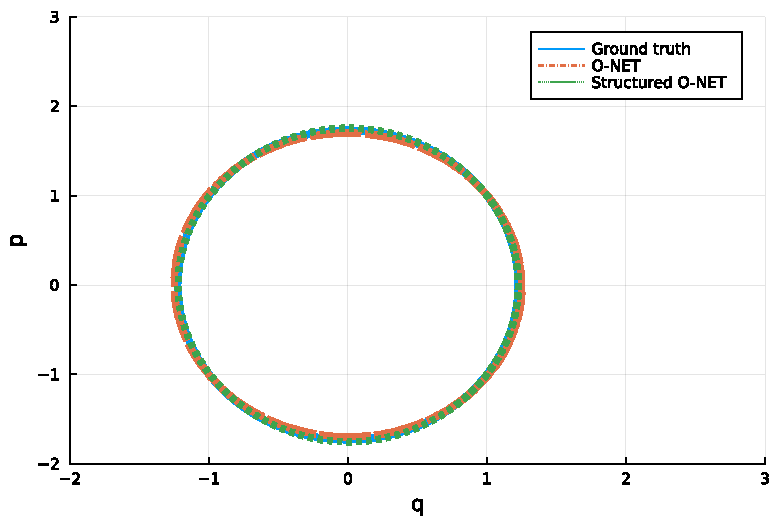
\includegraphics[scale=1]{figures/phase_portrait_O_NET.pdf}
    \caption{Phase portrait.}
    \label{fig:phase_portrait_O_NET}
\end{figure}

\begin{figure}[h!]
    \centering
    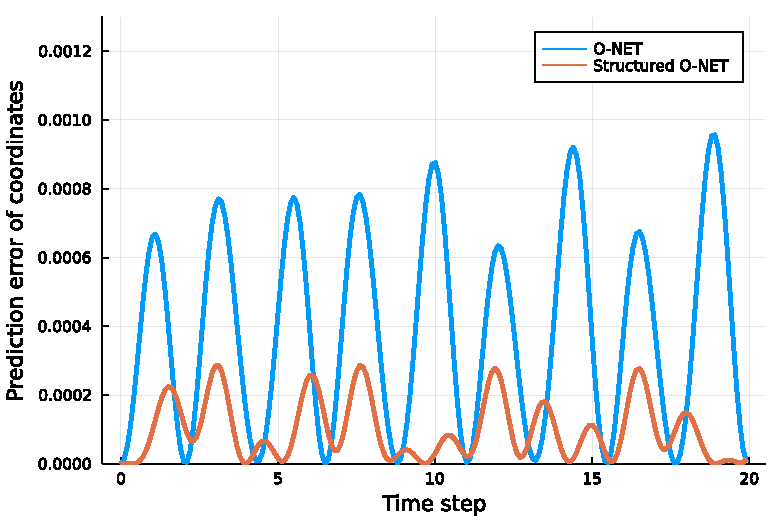
\includegraphics[scale=1]{figures/prediction_error_structured_O_NET.pdf}
    \caption{Prediction error.}
    \label{fig:prediction_error_structured_O_NET}
\end{figure}

\begin{figure}[h!]
    \centering
    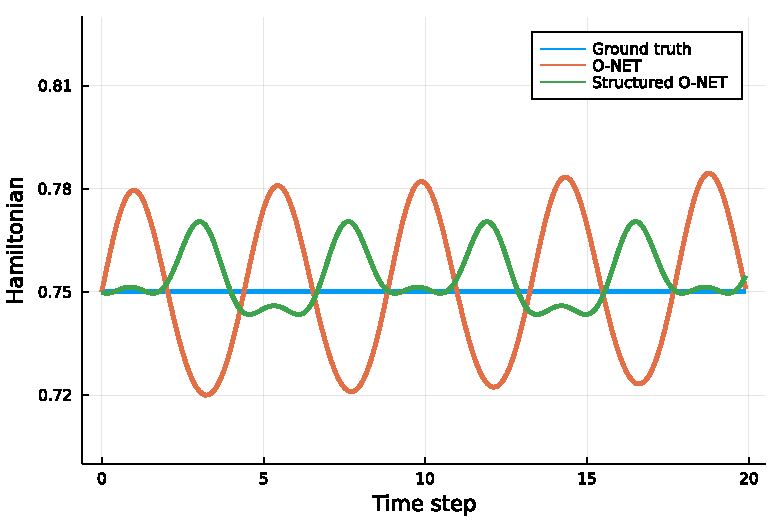
\includegraphics[scale=1]{figures/Hamiltonian_structured_O_NET.pdf}
    \caption{Time evolution of the total energy.}
    \label{fig:Hamiltonian_error_structured_O_NET}
\end{figure}

\begin{table}[h!]
	\centering
	\caption{Training and test error.}
	\label{tab:error_experiment1}
	\begin{tabularx}{\textwidth}{lcc}
		\toprule
		\textbf{Experiment 1} & \textbf{O-NET} & \textbf{Structured O-NET}\\
		\midrule
		Training error & $3.81\mathrm{e}{-4} \pm 0.57\mathrm{e}{-4}$ & $1.63\mathrm{e}{-4} \pm 0.15\mathrm{e}{-4}$ \\
		Test error & $7.75\mathrm{e}{-4} \pm 1.17\mathrm{e}{-4}$ & $4.38\mathrm{e}{-4} \pm 0.12\mathrm{e}{-4}$ \\
		\bottomrule
	\end{tabularx}
\end{table}



\clearpage
\section{Experiment: Isothermal Damped Harmonic Oscillator}
Unlike in experiment 1, an isothermal damped harmonic oscillator is a port-Hamiltonian system. The system of ODEs is of the form

\begin{equation}
    \label{eq:ODE_idho}
    \dot{x} =
    \begin{bmatrix}
    \dot{q}\\
    \dot{p}\\
    \end{bmatrix}
    =
    \begin{bmatrix}
    \frac{p}{m}\\
    -\frac{q}{c}-d\frac{p}{m}\\
    \end{bmatrix}.
\end{equation}

In the case of port-Hamiltonian systems, the total energy is not conserved. One might be more interested in irreversible components than reversible components. Hence, assume that the irreversible component $-d\frac{p}{m}$ is unknown and replace it with the output of a structured O-NET:

\begin{equation}
    \label{eq:structured_ODE_idho}
    \dot{x} =
    \begin{bmatrix}
    \dot{q}\\
    \dot{p}\\
    \end{bmatrix}
    =
    \begin{bmatrix}
    {f(q)}\\
    -\frac{q}{c} + {NN(p;\theta)}
    \end{bmatrix}
    =
    \begin{bmatrix}
    \frac{p}{m}\\
    -\frac{q}{c} + {NN(p;\theta)}\\
    \end{bmatrix}.
\end{equation}

In comparison to experiment 1, the RHS of $\dot{p}$ has both known part $-\frac{q}{c}$ and unknown part $NN(p;\theta)$. And the binary operator is $+$.

\textbf{Remark}. A special case of binary operation is division. If the known part is used as the numerator and the unknown part as the denominator, e.g., $\frac{f(t, x)}{NN(\mathbf{z}(t), t; \theta)}$, then one needs to add a constant $\varepsilon$ to the denominator to avoid instability, i.e., $\frac{f(t, x)}{NN(\mathbf{z}(t), t; \theta) + \varepsilon}$. This constant should be very small and not affect the learning result, e.g. $\varepsilon = 1 \times 10^{-8}$.

\textbf{Experiment Setup}.\\
Initial parameters: $m = 2.0, c = 1.0, d = 1.0$\\
Initial state: $x_0 = [1.0, 1.0]$\\
Time steps: $\{ 0.0, 0.1, 0.2, ..., 49.9 \}$\\
Gaussian Noise: $\sigma^2 = 0.01$\\
Integrator: implicit midpoint method\\
Optimization algorithm: ADAM

\clearpage
\begin{figure}[h!]
    \centering
    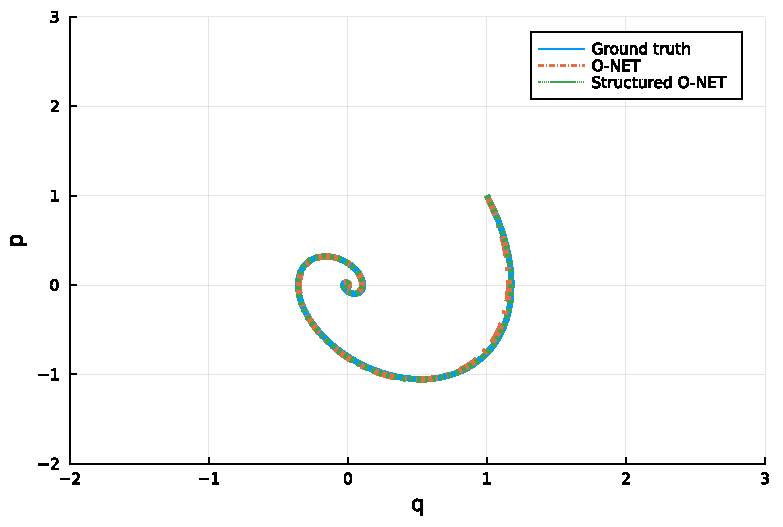
\includegraphics[scale=1]{figures/phase_portrait_O_NET_idho.pdf}
    \caption{Phase portrait.}
    \label{fig:phase_portrait_O_NET_idho}
\end{figure}

\begin{figure}[h!]
    \centering
    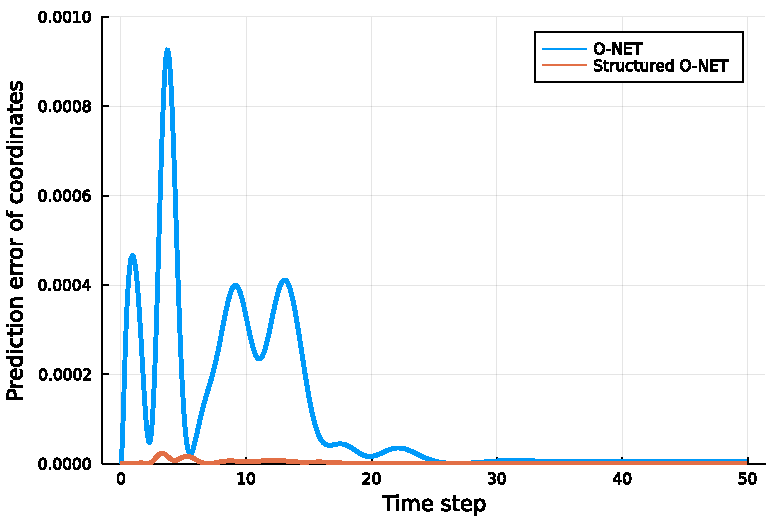
\includegraphics[scale=1]{figures/prediction_error_structured_O_NET_idho.pdf}
    \caption{Prediction error.}
    \label{fig:prediction_error_structured_O_NET_idho}
\end{figure}

\begin{figure}[h!]
    \centering
    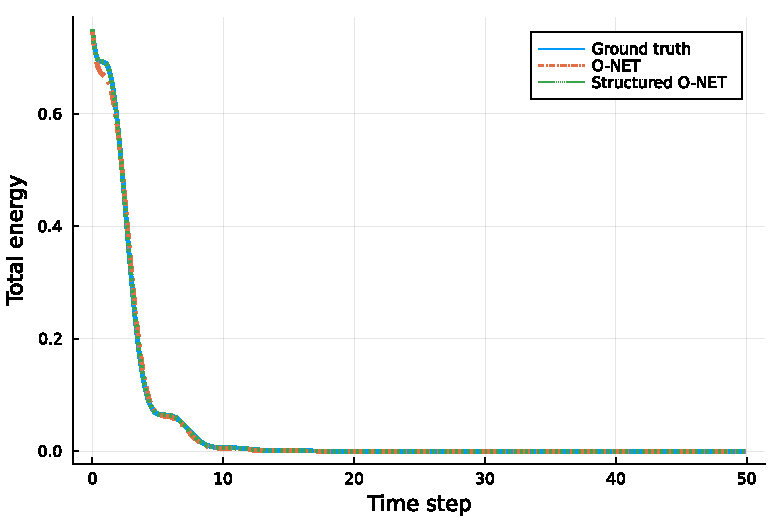
\includegraphics[scale=1]{figures/Hamiltonian_structured_O_NET_idho.pdf}
    \caption{Time evolution of the total energy.}
    \label{fig:Hamiltonian_error_structured_O_NET_idho}
\end{figure}

\begin{table}[h!]
	\centering
	\caption{Training and test error.}
	\label{tab:error_experiment2}
	\begin{tabularx}{\textwidth}{lcc}
		\toprule
		\textbf{Experiment 2} & \textbf{O-NET} & \textbf{Structured O-NET}\\
		\midrule
		Training error & $3.61\mathrm{e}{-4} \pm 1.28\mathrm{e}{-4}$ & $0.09\mathrm{e}{-4} \pm 0.07\mathrm{e}{-4}$ \\
		Test error & $6.94\mathrm{e}{-4} \pm 1.16\mathrm{e}{-4}$ & $2.88\mathrm{e}{-4} \pm 1.37\mathrm{e}{-4}$ \\
		\bottomrule
	\end{tabularx}
\end{table}

\clearpage
\chapter{Compositional Modelling}
\label{ch:chapter7}

As stated in the Port-Hamiltonian Systems chapter, a classical port-Hamiltonian system, e.g. an isothermal damped harmonic oscillator, can be depicted by a bond-graph expression \ref{fig:bondgraph_idho}. In \cite{lohmayer2021exergetic}, a thermodynamic modelling framework is proposed to extend a classical port-Hamiltonian system to an exergetic port-Hamiltonian system (EPHS). This modelling framework combines the classical port-Hamiltonian structure and the GENERIC framework, such that the EPHS is coherent with both the first and the second law of thermodynamics.

For an isothermal damped harmonic oscillator, its EPHS model can by expressed by the following bond-graph:

\begin{figure}[h!]
    \centering
    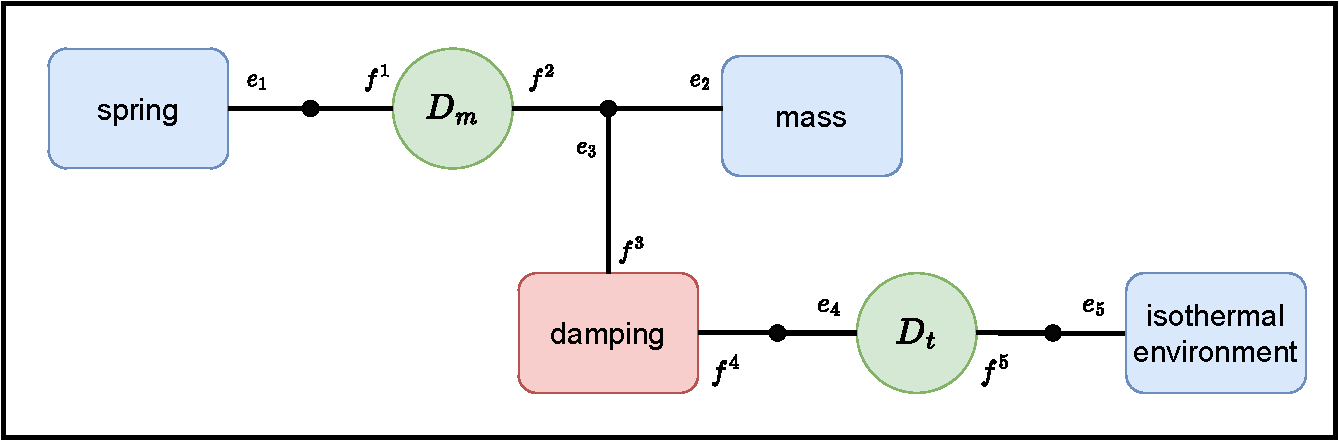
\includegraphics[scale=0.6]{figures/bondgraph_idho_exergetic.pdf}
    \caption{Bond-graph expression for defining an EPHS model of an isothermal damped harmonic oscillator.}
    \label{fig:bondgraph_idho_exergetic}
\end{figure}

However, following the assumption in the preceding chapter, there may be an unknown part in the system, which could be an obstacle to modeling. In this chapter, we propose a port-based modelling approach with structured O-NET. It combines with machine learning techniques and provides a new direction for compositional modelling.

For example, suppose that the resistive structure in red is the unknow part, the estimate of a neural network can be substituted for it:

\clearpage
\begin{figure}[h!]
    \centering
    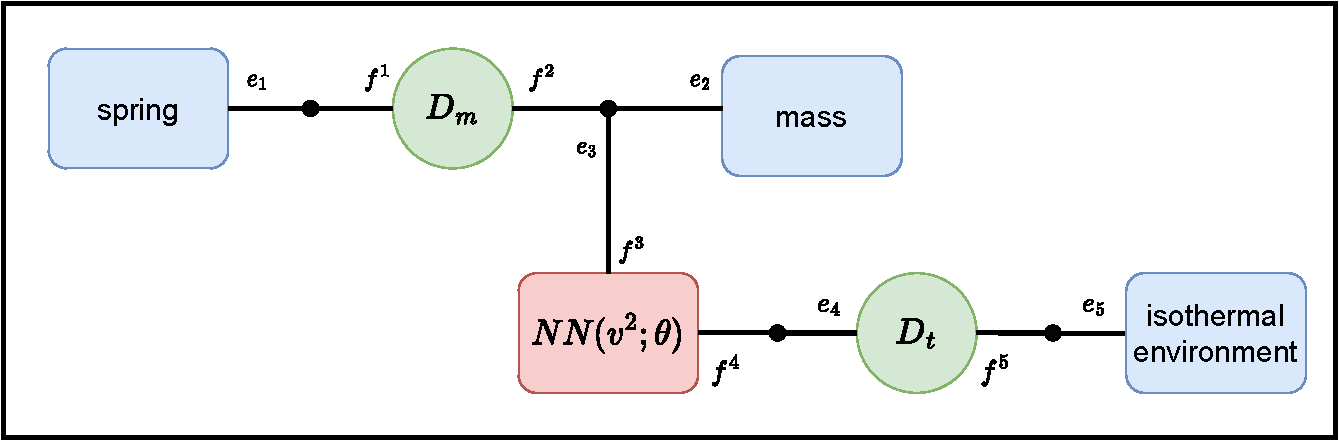
\includegraphics[scale=0.6]{figures/bondgraph_idho_exergetic_NN.pdf}
    \caption{Bond-graph expression for defining an EPHS model of an isothermal damped harmonic oscillator with neural network.}
    \label{fig:bondgraph_idho_exergetic_NN}
\end{figure}

The above model is a gray-box model, which is composed by the known part (storage components and Dirac structure) and the unknown part (resistive structure).


\section{Compositional Interconnection}

The subsystems in an isothermal damped harmonic oscillator interact with each other via interconnections:

\begin{equation}
    \label{eq:idho_interconnection1}
    \left[\begin{array}{c}
    f^1 \\
    f^2 \\
    \hline e_3
    \end{array}\right]=\left[\begin{array}{rr|r}
    0 & 1 & 0 \\
    -1 & 0 & -1 \\
    \hline 0 & 1 & 0
    \end{array}\right]\left[\begin{array}{c}
    e_1 \\
    e_2 \\
    \hline f^3
    \end{array}\right]
\end{equation}

\begin{equation}
    \label{eq:idho_interconnection2}
    \left[\begin{array}{c}
    f^5 \\
    \hline e_4
    \end{array}\right]=\left[\begin{array}{r|r}
    0 & -1 \\
    \hline 1 & 0
    \end{array}\right]\left[\begin{array}{c}
    e_5 \\
    \hline f^4
    \end{array}\right]
\end{equation}

\begin{equation}
    \label{eq:idho_interconnection3}
    \left[\begin{array}{l}
    f^3 \\
    f^4
    \end{array}\right]=\frac{1}{\theta_0} d\left[\begin{array}{rr}
    \theta_0 & -v \\
    -v & \frac{v^2}{\theta_0}
    \end{array}\right]\left[\begin{array}{l}
    e_3 \\
    e_4
    \end{array}\right],
\end{equation}

where $\theta_0$ is the environment temperature. And the system of ODEs can be expressed by

\begin{equation}
    \label{eq:ODE_idho_EPHS}
    \begin{bmatrix}
    \dot{q}\\\\
    \dot{p}\\\\
    \dot{s_e}
    \end{bmatrix}
    =
    \begin{bmatrix}
    \frac{p}{m}\\\\
    -\frac{q}{c}-d\frac{p}{m}\\\\
    \frac{1}{\theta_0} d v^2
    \end{bmatrix},
\end{equation}

where $s_e$ represents the environment entropy.

From the interconnections we can derive 

\begin{equation}
    \label{eq:flow}
    \begin{aligned}
    f^2 &= -e_1 - f^3\\
    f^5 &= \frac{e_3 f^3}{\theta_0}
    \end{aligned}
\end{equation}

In Figure \ref{fig:bondgraph_idho_exergetic_NN}, we replaced the resistive structure with the estimate of a neural network $ NN(v^2; \theta ) = e_3 f^3$, where the neural network takes the squared velocity $v^2$ as its input. Note that $v^2$ is a guess here, theoretically, $v$, $p$ or $(q, p)$ etc. can also be used as input. 

We construct a 1-input and 2-input neural network model, where the first output replaces $f^3$ and the second output replaces $e_3 f^3$. Plug the neural network into \ref{eq:flow}:

\begin{equation}
    \label{eq:flow_with_NN}
    \begin{aligned}
    f^2 &= -e_1 - NN(v;\theta)[1]\\
    f^5 &= \frac{NN(v^2;\theta)[2]}{\theta_0}
    \end{aligned}
\end{equation}

\section{Modelling with Structured O-NETs}

The neural network in \ref{eq:flow_with_NN} can be considered as a structured O-NET. Following \ref{eq:structured_O-NET_IVP}, the IVP of the above system can be defined by

\begin{equation}
    \label{eq:structured_O-NET_compositional_IVP}
    \dot{\mathbf{z}}_t = h_{\theta} \big(g(q, p), NN(v; \theta)[1], NN(v^2; \theta)[2] \big), \quad \mathbf{z}(t_{0}) = \mathbf{z}_{0} = [q, p, s],
\end{equation}

where $g(q, p)$ represents the known part (storage components and Dirac structure) and $NN(v^2; \theta)$ represents the unknown part (resistive structure).

In Julia code, we use the system of ODEs \ref{eq:ODE_idho_EPHS} to generate training set:

\begin{minted}[breaklines,escapeinside=||,mathescape=true, linenos, numbersep=3pt, gobble=2, frame=lines, fontsize=\small, framesep=2mm]{julia}
function ODEfunc_idho(dz, z, params, t)
    q, p = z
    m, c, d, θ_0 = params
    v = p/m
    dz[1] = v
    dz[2] = -q/c -d*v
    dz[3] = d*v^2/θ_0
end
\end{minted}

And the unknown part can be replaced by the estimate of a neural network:

\begin{minted}[breaklines,escapeinside=||,mathescape=true, linenos, numbersep=3pt, gobble=2, frame=lines, fontsize=\small, framesep=2mm]{julia}
m = 2
c = 1
θ_0 = 20
function ODE(df, z, θ, t)
    q = z[1]
    p = z[2]
    v = p/m
    dz[1] = v
    dz[2] = -q/c + Structured_O_NET([v], θ, st)[1][1]
    dz[3] = Structured_O_NET([v^2], θ, st)[1][2] / θ_0
end
\end{minted}

For the implementation in modelling, only the second output of the structured O-NET is needed, i.e., Structured\_O\_NET([$v^2$], θ, st)[1][2] $=$ $e_3 f^3 = dv^2$.

\section{Experiment: Isothermal Damped Harmonic Oscillator}


\begin{figure}[h!]
    \centering
    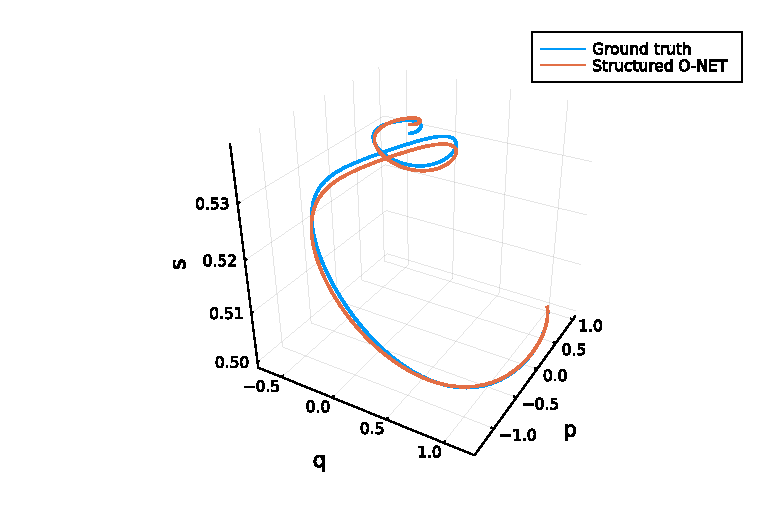
\includegraphics[scale=1]{figures/idho_phase_portrait.pdf}
    \caption{Phase portrait.}
    \label{fig:idho_phase_portrait}
\end{figure}

\clearpage
\begin{figure}[h!]
    \centering
    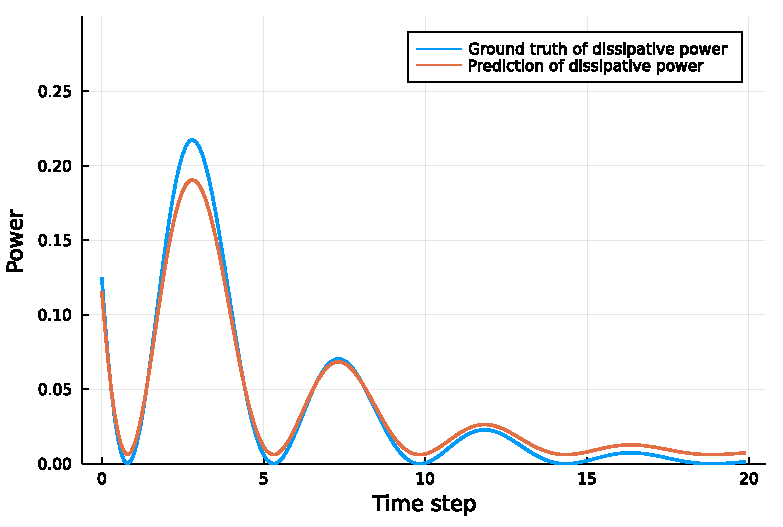
\includegraphics[scale=1]{figures/idho_dissipative_power.pdf}
    \caption{The time evolution of the dissipative power.}
    \label{fig:idho_dissipative_power}
\end{figure}

\begin{figure}[h!]
    \centering
    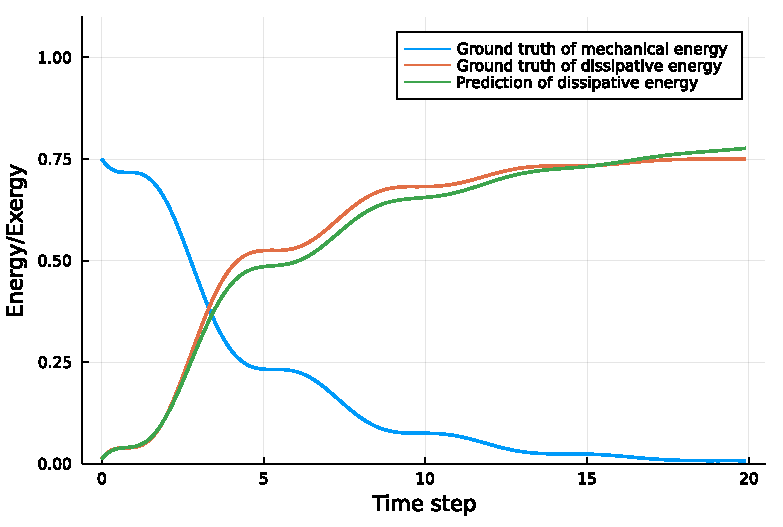
\includegraphics[scale=1]{figures/idho_energy_evolution.pdf}
    \caption{The time evolution of the energy/exergy.}
    \label{fig:idho_energy_evolution}
\end{figure}


\clearpage
\chapter{Conclusion}
\label{ch:chapter8}
\section{Summary}
\section{Outlook}


%%%%%%%%%%%%%%
% REFERENCES %
%%%%%%%%%%%%%%
\bibliographystyle{apalike}
\renewcommand{\bibname}{References} % Title References instead of Bibliography
\bibliography{literature/literature}


%%%%%%%%%%%%
% APPENDIX %
%%%%%%%%%%%%
\appendix


\end{document}